\documentclass[12pt]{amsart}

\RequirePackage[OT1]{fontenc}

\usepackage[foot]{amsaddr}
% \usepackage{biblatex}
\usepackage{natbib}
%\bibliographystyle{apalike}
\usepackage{multirow}
\usepackage{enumitem}
\usepackage{caption,subcaption}

\usepackage{xr}
\makeatletter
\newcommand*{\addFileDependency}[1]{% argument=file name and extension
  \typeout{(#1)}% latexmk will find this if $recorder=0 (however, in that case, it will ignore #1 if it is a .aux or .pdf file etc and it exists! if it doesn't exist, it will appear in the list of dependents regardless)
  \@addtofilelist{#1}% if you want it to appear in \listfiles, not really necessary and latexmk doesn't use this
  \IfFileExists{#1}{}{\typeout{No file #1.}}% latexmk will find this message if #1 doesn't exist (yet)
}
\makeatother

\newcommand*{\myexternaldocument}[1]{%
    \externaldocument{#1}%
    \addFileDependency{#1.tex}%
    \addFileDependency{#1.aux}%
}
%%% END HELPER CODE

% put all the external documents here!
\myexternaldocument{covid-writeup}



\usepackage{tchdr}
\boldshortcuts

\usepackage{url}

\usepackage{graphicx}
\usepackage{wrapfig}
\usepackage{setspace}
\DeclareGraphicsExtensions{.eps, .ps}
\usepackage{amsmath, amsthm, amsfonts}
% \usepackage[margin=1.5in]{geometry}

\numberwithin{equation}{section}
\theoremstyle{plain}
\newtheorem{theorem}{Theorem}[section]
% \newtheorem{example}{Example}
% \newtheorem{remark}{Remark}
\newtheorem{corollary}[theorem]{Corollary}
\newtheorem{criterion}[theorem]{Criterion}
\newtheorem{definition}[theorem]{Definition}
\newtheorem{exercise}[theorem]{Exercise}
\newtheorem{lemma}[theorem]{Lemma}
\newtheorem{proposition}[theorem]{Proposition}

\setlength{\textwidth}{6.5in}
\setlength{\textheight}{8.5in}
\setlength{\topmargin}{-0.25in}
\setlength{\evensidemargin}{0in}
\setlength{\oddsidemargin}{0in}
%\setlength{\evensidemargin}{.25in}
%\setlength{\oddsidemargin}{.25in}


\usepackage{setspace}
% \onehalfspacing
\doublespacing


\def\logit{\text{logit}}
\def\pr{\text{pr}}
\def\sgn{\text{sgn}}
\def\I{\bf I}
\def\code#1{\texttt{#1}}
\def\EE{\mathbb{E}}
%\newcommand{\indep}{\perp \!\!\! \perp}

\begin{document}

\title[Statistical paradoxes in coronavirus case-counts]{Supplementary Materials to ``Statistical paradoxes in coronavirus case-counts: selection bias, measurement error, and the COVID-19 pandemic''} %

\author{Walter Dempsey}
\address{Department of Biostatistics, University of Michigan, Ann Arbor, MI 48109}
% \email{wdem@umich.edu}

\begin{abstract}
This is the supplementary materials to the manuscript titled ``Statistical paradoxes in coronavirus case-counts: selection bias, measurement error, and the COVID-19 pandemic.''  Section~\ref{app:imperfect} derives the statistical decompositions for the measurement-error corrected estimator and provides the connection to model-based estimators. Sections~\ref{app:ipwderivation} and~\ref{app:DRderivation} derives the statistical decomposition for the inverse-probability weighted and doubly robust estimators respectively.
Section~\ref{app:asympderivations} gives the proof for the asymptotics of the inverse-probability weighted estimator.  
Section~\ref{app:irls} outlines the iteratively re-weighted least squares algorithm.
Section~\ref{app:in_add_details} provides additional detals on the COVID-19 analysis of Indiana's case-count data.
Section~\ref{app:prior_modelbased} provides prior specifications for the SEIR model.
\end{abstract}

\maketitle

\newpage
\appendix

\section{Reproducible code}

All relevant code can be found at \url{https://github.com/wdempsey/covid-umich}.

\section{Notation Glossary}
\label{app:notation}

\paragraph{Notation for Section~\ref{section:casecount} (non-temporal setting)}
\begin{itemize}
\item[$Y_j$] \quad Binary COVID-19 status of individual $j$ in the population.
\item[$N$] \quad Population size
\item[$\bar Y$] \quad Population average, $\bar Y = N^{-1} \sum_{j=1}^N Y_j$
\item[$I_j$] \quad Selection indicator of individual $j$ in the population into the sample
\item[$y_j$] \quad Binary COVID-19 status of sample individual $j=1,\ldots,n$.
\item[$\bar y_n$] \quad Sample average, $\bar y_n = n^{-1} \sum_{j=1}^N I_j Y_j = n^{-1} \sum_{j=1}^n y_j$
\item[$\rho_{I,Y}$] \quad \emph{Data quality}, i.e., correlation between selection indicator and population outcome
\item[$f$] \quad \emph{Data quantity}, i.e., sampling fraction $f = n/N$
\item[$\sigma_Y$] \quad \emph{Problem Difficulty}, i.e., population variance $\sigma_Y^2 = (N)^{-1} \sum_{j=1}^N (Y_j - \bar Y)^2$.
\item[$FP$] \quad False Positive Rate
\item[$FN$] \quad False Negative Rate
\item[$\tilde y_n$] \quad Sample average adjusted for false negative and positive rates, i.e., $\tilde y_n = (1-FP-FN)^{-1} (\bar y_n - FP)$
\item[$f_0, f_1$] \quad Sampling fraction among COVID-19 negative and positive individuals respectively, i.e., $f_1 := \sum_{j=1}^N I_j Y_j / \sum_{j=1}^N Y_j$
and $f_0 := \sum_{j=1}^N I_j (1-Y_j) / \sum_{j=1}^N (1-Y_j)$.
\item[$\Delta, M$] \quad Sampling rate differential on additive -- $\Delta = f_1 - f_0$ -- and multiplicative -- $M = f_1/f_0$ -- scales.
\end{itemize}

\paragraph{\bf Notation for Section~\ref{section:improvedcasecount} (temporal setting)}
\begin{itemize}
\item[$Y_{j,t}$] \quad Binary COVID-19 status of individual $j$ in the population at time~$t$.
\item[$I^{NR}_{j,t}$] \quad Selection indicator of individual $j$ in the population into the non-probability sample.
\item[$X_{j,t}$] \quad Feature vector for individual $j$ in the population at time~$t$ that impact self-selection into the non-probability sample.
\item[$I_{j,t}^{R}$] \quad Selection indicator of individual $j$ in the population into the probability sample.
\item[$W_{j,t}^{R}$] \quad Weight of individual $j$ in the population in the probability sample (i.e., inverse-probability of selection)
\item[$\pi (X_{j,t}; \theta)$] \quad Self-selection propensity of individual~$j$ into the non-probability sample given feature vector~$X_{j,t}$ and parameter~$\theta$.
\item[$w (X_{j,t})$] \quad Weight of individual~$j$ in the population in the non-probability sample, i.e., $w(x) = 1/\pi(x; \theta)$.
\item[$\hat \mu(X_{j,t})$] \quad Model-based estimate of the active infection rate at time~$t$ for individuals with feature vector~$X_{j,t}$
\end{itemize}

\section{Technical details}

Recall that $P_j$ is  an indicator of measurement error, equal to $1$ when we incorrectly measure the outcome and $0$ when we observe the true outcome. We suppose this is a stochastic variable where $\pr(P_j = 1 \mid Y_j = 1) =: FN$ is the false-negative rate and $\pr(P_j = 1 \mid Y_j = 0) =: FP$ is the false-positive rate.  If individual $j$ is selected (i.e., $I_j = 1$) then the observed outcome can be written as $Y_j^{\star} = Y_j(1-P_j) + (1-Y_j) P_j$.

\subsection{Derivations for imperfect testing framework.}
\label{app:imperfect}
We start by considering the empirical mean estimator under imperfect testing,
$$
\bar y_n^\star = \frac{\sum_{j=1}^N Y_j^\star I_j}{\sum_{j=1}^N I_j} = \frac{\sum_{i=1}^N  I_j Y_j^\star }{\sum_{j=1}^N  I_j } = \frac{\sum_{i=1}^N  I_j \left[ Y_j (1-P_j) + (1-Y_j) P_j \right]}{\sum_{j=1}^N  I_j }
$$
For any set of numbers $\{ A_1, \ldots, A_N \}$ we can view it as the support of a random variable $A_J$ induced by the random index $J$ defined on $\{1,\ldots, N\}$.  When $J$ is uniformly distributed $E_J (A_J) = \sum_{j=1}^N A_j / N \equiv \bar A_N$. Then
$$
\begin{aligned}
\bar y_n^\star  - \bar Y_N &= \frac{E_J \left[ I_J \left[ Y_J (1-P_J) + (1-Y_J) P_J \right] \right]}{E_J [ I_J ] } - E_J[Y_J] \\
&= \frac{E_J \left[ I_J P_J (1-2Y_J) \right]}{E_J [ I_J ] } + \left( \frac{E_J [I_J Y_J]}{E_J [ I_J ] } - \frac{E_J[Y_J] E_J[I_J]}{E_J[I_J]} \right) \\
\end{aligned}
$$
The term in parentheses can be re-written as
$$
\begin{aligned}
\frac{E_J [I_J Y_J]- E_J[Y_J] E_J[I_J]}{E_J[I_J]} &=  \frac{E_J [I_J Y_J]- E_J[Y_J] E_J[I_J]}{\sqrt{V_J(I_J) V_J(Y_J)}} \frac{\sqrt{V_J(I_J)}}{E_J[I_J]} \times \sqrt{V_J(Y_J)} \\
&= \rho_{I,Y} \times \sqrt{\frac{(1-f)}{f}} \times \sigma_Y
\end{aligned}
$$
which agrees with Meng's (2019) decomposition. For the other term, first we define $Z_j := 1 - 2 Y_j $. Then $Z_j = 1$ if $Y_j = 0$ and $Z_j = -1$ if $Y_j = 1$. Then the term can be re-written as
$$
\begin{aligned}
\frac{E_J \left[ I_J P_J (1-2Y_J) \right]}{E_J [ I_J ] } &= \left( \frac{E_J \left[ I_J P_J Z_J \right]}{E_J [ I_J ] } -  \frac{E_J \left[ P_J Z_J \right] E_J[ I_J]}{E_J [ I_J ] } \right) +  \frac{E_J \left[ P_J Z_J \right] E_J[ I_J]}{E_J [ I_J ] } \\
\end{aligned}
$$
The term in parentheses can be re-expressed using the previous technique as:
$$
\rho_{I, PZ} \times \sqrt{\frac{1-f}{f}} \times \sigma_{PZ}
$$
where now the ``data defect'' and ``problem difficulty'' are with respect to $PZ$ rather than $Y$. The final term is equal to
$$
\begin{aligned}
E_J [P_J Z_J ] &= E_J [ E_J [ P_J Z_J \mid Y_J ] ] \\
&= \pr (P = 1 \mid Y = 0) (1-\bar Y) - \pr(P=1 \mid Y = 1) \bar Y \\
&= FP - (FP + FN) \cdot \bar Y
\end{aligned}
$$
Combining these yields:
$$
\bar y_n^\star - \bar Y = \sqrt{\frac{1-f}{f}} \left(\rho_{I,Y} \sigma_Y + \rho_{I, PZ} \sigma_{PZ} \right) + \left( FP - (FP+FN) \bar Y \right)
$$

\subsubsection{Derivation of an estimator unbiased under SRS}
\label{app:memestimator}
We see the final term is given by $FP (1-\bar Y) - FN \bar Y$ is the bias associated with using the unadjusted prevalence estimate $\bar y_n^\star$.  This motivates an adjusted estimate
$$
\tilde y_n^{(0)} = \bar y_n^\star - FP (1- \bar y_n^\star ) + FN \bar y_n^\star
= \bar y_n^\star (1 + FN + FP) - FP.
$$
Now considering the error for the adjusted estimate, $\tilde y_n^{(0)} - \bar Y$, we have
$$
\begin{aligned}
 &\bar y_n^\star (1 + FN + FP) - FP - \bar Y \\
 =&(\bar y_n^\star - \bar Y) +  (FN + FP) \bar y_n^\star - FP  \\
 =&\underbrace{\sqrt{\frac{1-f}{f}} \left[\rho_{I,Y} \sigma_Y + \rho_{I, PZ} \sigma_{PZ} \right]}_{\Psi} + (  FN + FP ) (\bar y_n^\star -  \bar Y) \\
 =& \Psi + (FN + FP) \Psi + (FN + FP) (FP - (FP+FN) \bar Y).
 \end{aligned}
$$
The final term is a (smaller) bias term and so we propose another adjusted estimator $\tilde y_n^{(1)} = \tilde y_n^{(0)} + (FN+FP)  ( (FN+FP) \bar y_n^\star - FP)$, with associated error $\tilde y_n^{(1)} - \bar Y$ given by
$$
\begin{aligned}
 &(\bar y_n^{(0)} - \bar Y) + (FN+FP)  ( (FN+FP) \bar y_n^\star - FP)\\
 =&\Psi + (FN + FP) \Psi + (FN + FP) (FP - (FP+FN) \bar Y) + (FN + FP) ((FP+FN) \bar y_n^\star - FP)  \\
  =& \Psi + (FN + FP) \Psi + (FN + FP)^2 \Psi + (FN+FP)^2 (FP - (FP+FN) \bar Y).
 \end{aligned}
$$
This motivates recursively defining estimators $\tilde y_n^{(t)} = \tilde y_n^{(t-1)} + (FN+FP)  ( (FN+FP) \bar y_n - FP)$ for $t=1,2,\ldots$ where $\tilde y_n^{(0)} = \bar y_n^\star$.  Then
$$
\tilde y_n^{(t)} = \bar y_n^\star \sum_{s=0}^{t+1} (FP+FN)^s - FP \sum_{s=0}^{t} (FP+FN)^s
$$
and the associated error at iteration $t$ given by
$$
\Psi \sum_{s=0}^t (FN+FP)^s = \Psi \frac{1 - (FN+FP)^t}{1 - (FN+FP)}.
$$
We can then get an estimator with no residual bias term by taking the limit as $t$ goes to infinity; that is, define
$$
\tilde y_n = \lim_{t \to \infty} \tilde y_n^{(t)} = \frac{\bar y_n^\star - FP}{1 -(FN+FP)}.
$$
Then the associated error $\tilde y_n - \bar Y$ can be expressed as $\frac{\Psi}{1-(FN+FP)}$.

\subsection{Model-based derivation of the estimator.}
\label{app:modelbased}
The estimator $\tilde y$ was derived as a limit of a process that removes the residual bias term at each step.  Here we consider a model-based explanation.  Let $\theta = \pr( Y = 1)$ and $\phi = \pr( \text{test is positive})$.  Given a known false negative (FN) and false positive (FP) rates, we have
$$
\begin{aligned}
\phi &= \theta \cdot (1-FN) + (1-\theta) \cdot FP = \theta (1-FN-FP) + FP \\
\Rightarrow \theta &= \frac{\phi - FP}{1-FN-FP}.
\end{aligned}
$$
Thus, the estimator $\tilde y$ is also the appropriate estimator under a model-based approach.  While the derivation here is more straightforward, the derivation in the prior section provides a simple formula for the associated error $\tilde y_n - \bar Y$ and gives a novel connection between the empirical estimator $\bar y_n^\star$ and the adjusted estimator $\tilde y_n$ without reference to the model-based approach.

\subsection{Further simplification.}
For the binary outcome $Y$, we have $\sigma_Y = \sqrt{\bar Y (1-\bar Y)}$. Moreover,
$$
\begin{aligned}
V_J(P_J Z_J) &= E_J[(P_J Z_J)^2] - E_J[P_J] E_J[Z_J] \\
&= E_J[P_J] - E_J[P_J] (1 - 2 \bar Y) = 2 \bar Y E_J [ P_J ] \\
&= 2 \bar Y \left( FP (1-\bar Y) + FN \bar Y \right) \\
\Rightarrow \sigma_{PZ} &= \sqrt{ 2 \bar Y \left( FP (1-\bar Y) + FN \cdot  \bar Y \right) }
\end{aligned}
$$
Then the formula for the error is given by:
\begin{equation}
\label{eq:finalstep}
\sqrt{\frac{1-f}{f}} \left[\rho_{I,Y} \sqrt{\bar Y (1-\bar Y)} + \rho_{I, PZ} \sqrt{ 2 \bar Y \left( FP (1-\bar Y) + FN \cdot \bar Y \right )} \right] \times \frac{1}{1- (FN+FP)}
\end{equation}
By definition, we have
$$
\begin{aligned}
\rho_{I,PZ} &= \frac{C(I, PZ)}{\sqrt{V(PZ) V(I)}} \\
&= \frac{C(I, PZ)}{\sqrt{V(Y) V(I)}} \sqrt{\frac{V(Y)}{V(PZ)}} \\
&= \rho_{I,Y} \frac{C(I,PZ)}{C(I,Y)} \sqrt{ \frac{(1-\bar Y)}{2 ( FP (1-\bar Y) + FN \cdot \bar Y)} }
\end{aligned}
$$

$$
\begin{aligned}
C(I, PZ) &= E[ I P Z ] - E[I] E[PZ] \\
&=  [FP f_0 - (FP f_0 + FN f_1) \bar Y] - f [ FP - (FP+FN) \bar Y ] \\
&=  - FP \Delta \bar Y + FP \bar Y^2 \Delta - FN \bar Y^2 \Delta \\
&=  - \Delta \bar Y (FP \cdot (1-\bar Y) + FN \cdot \bar Y) \\
\end{aligned}
$$
where $f = f_1 \bar Y + f_0 (1-\bar Y)$ so $f_0 - f = -\Delta \bar Y$ and $f_1 - f = \Delta (1-\bar Y)$.
$$
\begin{aligned}
C(I, Y) &= E[ I Y ] - f \bar Y \\
&=  f_1 \bar Y + f_0 (1-\bar Y) - f \bar Y \\
&=  f_0 (1-\bar Y) + \Delta (1-\bar Y) \bar Y \\
&= (1-\bar Y) (f_0 + \Delta \bar Y)
\end{aligned}
$$
Combining yields
$$
\begin{aligned}
\rho_{I,PZ} &= \rho_{I,Y} \times \frac{- \Delta \bar Y (FP \cdot (1-\bar Y) + FN \cdot \bar Y) }{(1-\bar Y) (f_0 + \Delta \bar Y)} \times \sqrt{ \frac{(1-\bar Y)}{2 ( FP (1-\bar Y) + FN \cdot \bar Y)} } \\
&= - \rho_{I, Y} \times \Delta \times \sqrt{\frac{\bar Y}{1-\bar Y}} \frac{\sqrt{FP(1-\bar Y) + FN \cdot \bar Y}}{f_0 (1-\bar Y) + f_1 \bar Y} \times \sqrt{\frac{\bar Y}{2}}
\end{aligned}
$$
We can then re-write $\rho_{I,Y} \sigma_Y + \rho_{I,PZ} \sigma_{PZ}$ as
$$
\rho_{I,Y} \sigma_Y \left( 1 - \Delta \times \frac{\bar Y}{1-\bar Y} \times \frac{FP(1-\bar Y) + FN \cdot \bar Y}{f_0 (1-\bar Y) + f_1 \bar Y} \right).
$$
Inserting into equation~\eqref{eq:finalstep} yields the desired result.

\subsection{Derivation of effective sample size}
\label{app:effss}

Let $S_Y^2 = (N-1)^{-1} \sum_{j=1}^N (Y_j - \bar Y)^2$ be the population variance as defined in survey sampling~\citep{Cochran77}.  Then $\sigma_Y^2 = (N-1)/N \cdot S_Y^2$.  Under SRS, the MSE is the variance as the estimate is unbiased and the variance is given by $(1-f)/n S_Y^2$.  Then setting the MSE under general selection and SRS equal we have
$$
\begin{aligned}
\underbrace{\frac{1-f}{f} \times E_{\I} \left[ \rho_{I, Y}^2 \times D_M^2 \right]}_{1/n_{eff}^\star} \times \sigma_Y^2 &= \frac{1-f}{n_{eff}} S_Y^2 \\
\frac{1}{n_{eff}^\star} \times \frac{N-1}{N} S_Y^2 &= \frac{1-f}{n_{eff}} S_Y^2 \\
\frac{1}{n_{eff}^\star} &=  \left( \frac{1}{n_{eff}} - \frac{1}{N} \right) \left( \frac{N}{N-1} \right) \\
\frac{1}{n_{eff}^\star} \left[ 1 - \frac{1}{N} + \frac{n_{eff}^\star}{N} \right]  &=  \frac{1}{n_{eff}} \\
n_{eff}^\star \left[ 1 - \frac{1}{N} + \frac{n_{eff}^\star}{N} \right]^{-1}  &=  n_{eff} \\
\frac{n_{eff}^\star}{ 1 + (n_{eff}^\star -1) N^{-1}} &=  n_{eff} \\
\end{aligned}
$$
Then if $n_{eff}^\star \geq 1$, we have that
$$
n_{eff} \leq n_{eff}^\star = \frac{f}{1-f} \times \frac{1}{E_{\I} \left[ \rho^2_{I, Y} \times D_M^2 \right]}
$$

\subsection{Ratio estimator}
\label{app:ratio}

Let ${\bf u} = (u_{t-1},u_t) \in \mathbb{R}^2$ and $g({\bf u}) = \frac{u_t}{u_{t-1}}$, i.e., a differentiable function $g:\mathbb{R}^2 \to \mathbb{R}$. Centering a Taylor series expansion of second-order around coordinates $(U_2, U_1) \in \mathbb{R}^2$ yields
$$
\begin{aligned}
g({\bf u}) =& g(U_{t-1}, U_t) - \frac{U_t}{U_{t-1}^2} (u_{t-1} - U_{t-1}) + \frac{1}{U_{t-1}} (u_t - U_t) \\
&+ \frac{1}{2} \left[ \frac{2 U_t}{U_{t-1}^3} (u_{t-1} - U_{t-1})^2 + 0 \times (u_t - U_t)^2 - 2 \times (u_{t-1} - U_{t-1}) (u_t - U_t) \frac{1}{U_t^2} \right]
\end{aligned}
$$
Plugging in $(\bar y_{t-1}, \bar y_t)$ for $(u_{t-1}, u_t)$ and $(\bar Y_{t-1}, \bar Y_t)$ for $(U_{t-1}, U_t)$ yields the $\frac{\bar y_t}{\bar y_{t-1}} - \frac{\bar Y_t}{\bar Y_{t-1}} $ is equal to
$$
\begin{aligned}
=&
- \frac{\bar Y_t}{\bar Y_{t-1}^2} (\bar y_{t-1} - \bar Y_{t-1}) + \frac{1}{\bar Y_{t-1}} (\bar y_t - \bar Y_t) \\
&+ \frac{\bar Y_t}{\bar Y_{t-1}^3} (\bar y_{t-1} - \bar Y_{t-1})^2 -  (\bar y_{t-1} - \bar Y_{t-1}) (\bar y_t - \bar Y_t) \frac{1}{\bar Y_{t-1}^2} \\
&= \frac{\bar Y_t}{\bar Y_{t-1}} \bigg[  \rho_{I_t,Y_t} \sqrt{\frac{1-f_t}{f_t}} CV (Y_t)  -\rho_{I_{t-1},Y_{t-1}} \sqrt{\frac{1-f_{t-1}}{f_{t-1}}} CV (Y_{t-1}) \\
&+ \rho^2_{I_{t-1},Y_{t-1}} \frac{1-f_{t-1}}{f_{t-1}} CV^2 (Y_{t-1}) -  \rho_{I_{t-1},Y_{t-1}} \sqrt{\frac{1-f_{t-1}}{f_{t-1}}} CV (Y_{t-1}) \times
\rho_{I_t,Y_t} \sqrt{\frac{1-f_t}{f_t}} CV (Y_t)   \bigg] \\
&= \frac{\bar Y_t}{\bar Y_{t-1}} \bigg[ \rho_{I_t,Y_t} \sqrt{\frac{1-f_t}{f_t}} CV (Y_t)  -\rho_{I_{t-1},Y_{t-1}} \sqrt{\frac{1-f_{t-1}}{f_{t-1}}} CV (Y_{t-1}) \bigg] \left[ 1 - \rho_{I_{t-1},Y_{t-1}} \sqrt{\frac{1-f_{t-1}}{f_{t-1}}} CV (Y_{t-1}) \right]
\end{aligned}
$$
where the second equality is obtained by plugging in the statistical decomposition of the error for both time points and the coefficient of variation being defined as $CV(Y) := \sigma_Y/\mu_Y$.  Under measurement error, the extra terms $D_{t}$ and $D_{t-1}$ can be inserted in the correct locations.

\subsection{Estimation of effective reproduction number}

Let
$$
\delta_t := \bigg[ \rho_{I_t,K_t} D_{M_t} \sqrt{\frac{1-f_t}{f_t}} CV (K_t)  -\rho_{I_{t-1},K_{t-1}} D_{M_{t-1}} \sqrt{\frac{1-f_t}{f_t}} CV (K_{t-1}) \bigg].
$$
Then the previous sections derivation shows that the estimate of the number of new cases on day t is given by
$$
\frac{S_t \cdot \bar y_t}{S_{t-1} \cdot \bar y_{t-1}} =
\frac{K_t}{K_{t-1}} \left( 1 + \delta_t \times \left[ 1 - \rho_{I_{t-1},K_{t-1}} D_{M_{t-1}} \sqrt{\frac{1-f_t}{f_t}} CV (K_{t-1}) \right] \right)
$$
Then setting $e_t = \delta_t \times [1 - \rho_{I_{t-1},K_{t-1}} D_{M_{t-1}} \sqrt{\frac{1-f_t}{f_t}} CV (K_{t-1}) ]$, we have
$$
\begin{aligned}
\log \left( \frac{S_t \bar y_t}{S_{t-1} \bar y_{t-1}} \right) - \log \left( \frac{K_t}{K_{t-1}} \right) &= \log (1 + e_t) \\
\log \left( \frac{\bar y_t}{\bar y_{t-1}} \right) - \log \left( \frac{K_t}{K_{t-1}} \right) &= 1 + e_t - \log \left( \frac{S_t}{S_{t-1}} \right) \\
1 + \frac{1}{\gamma} \log \left( \frac{\bar y_t}{\bar y_{t-1}} \right) - \left[ 1 + \frac{1}{\gamma} \log \left( \frac{K_t}{K_{t-1}} \right) \right] &= \frac{1}{\gamma} \left[ \log \left( 1 + e_t \right) - \log \left( \frac{S_{t}}{S_{t-1}} \right) \right] \\
\Rightarrow \hat R_t - R_t &= \frac{1}{\gamma} \left[ \log \left( 1 + e_t \right) - \log \left( \frac{S_{t}}{S_{t-1}} \right) \right]
\end{aligned}
$$

\subsection{Computing the effective sample size}
\label{section:effss}

For binary outcomes, we have
\begin{equation} \label{eq:binaryrho}
\rho_{I,Y} = \Delta \sqrt{\frac{\bar Y (1 - \bar Y)}{f (1-f)} }
\end{equation}
where $\Delta = P_J (I_J = 1 \mid Y_J = 1) - P(I_J = 1 \mid Y_J = 0) = f_1 - f_0$.  Suppose that $M = f_1/f_0$; then $f_0 = f / (\bar Y \cdot (M-1) + 1)$.  Using the upper bound $E_{\I} [ \rho_{I,Y}^2 ] \leq E_{\I} [\rho_{I,Y} ]^2$, we compute effective sample size under a range of prevalences $\bary$, and relative sample rates $M$ given $f = 0.003$ (i.e., current sampling fraction).

\begin{table}[ht]
\centering
\begin{tabular}{rrrrrrrr}
& \multicolumn{7}{c}{$M$} \\ \cline{2-8}
$\bar y$ & 1.05 & 1.15 & 1.25 & 1.35 & 1.45 & 1.55 & 1.65 \\
  \hline
0.01 & 40444 & 4503 & 1624 & 830 & 503 & 338 & 242 \\
0.03 & 13787 & 1541 & 558 & 286 & 174 & 117 & 85 \\
0.05 & 8463 & 950 & 345 & 178 & 109 & 73 & 53 \\
0.07 & 6187 & 697 & 254 & 132 & 81 & 55 & 40 \\
0.09 & 4928 & 557 & 204 & 106 & 65 & 44 & 32 \\
0.11 & 4131 & 469 & 173 & 90 & 56 & 38 & 28 \\
   \hline
\end{tabular}
\end{table}

We also present the same plot under $FP = 0.024$ and $FN = 0.13$ to show the impact of measurement error on effective sample size.

\begin{table}[ht]
\centering
\begin{tabular}{rrrrrrrr}
& \multicolumn{7}{c}{$M$} \\ \cline{2-8}
 & 1.05 & 1.15 & 1.25 & 1.35 & 1.45 & 1.55 & 1.65 \\
  \hline
0.01 & 29019 & 3247 & 1177 & 605 & 368 & 248 & 179 \\
0.03 & 9894 & 1112 & 405 & 209 & 128 & 87 & 63 \\
0.05 & 6075 & 686 & 251 & 130 & 80 & 54 & 39 \\
0.07 & 4442 & 504 & 185 & 96 & 59 & 41 & 30 \\
0.09 & 3539 & 403 & 149 & 78 & 48 & 33 & 24 \\
0.11 & 2967 & 339 & 126 & 66 & 41 & 28 & 21 \\
   \hline
\end{tabular}
\end{table}

For binary outcomes, we have
\begin{equation} \label{eq:weightedbinaryrho}
\rho_{\tilde I (X),Y} = \tilde \Delta \sqrt{\frac{\bar Y (1 - \bar Y)}{f (1-f) \text{E}(W_J \mid I_J = 1)^2 + f \text{Var}(W_J \mid I_J = 1)} }
\end{equation}

% \section{Effect modifiers in COVID-19 clinical trials}

% Here we show how selection bias and measurement error can creep into clinical trial analysis. The key concern is whether clinical trials on COVID-19 recruit from the pool of individuals who have tested positive for COVID-19 or whether they sample randomly from the population, test, and then recruit from this subset of tested individuals.  To see this issue, suppose we have an outcome $Y$, a treatment $A$ and an \emph{unobserved} variable $U$.  Suppose treatment is assigned at random, i.e., $A =1$ with probability $50\%$ and $A=0$ with probability $50\%$.  Suppose the conditional mean of the outcome satisfies  $E(Y \mid U, A ) = \beta_0 + \beta_1 A + \beta_2 U + \beta_3 A U$.  Typically, we are interested in the \emph{causal effect} of $A$ on $Y$.  In counterfactual language,
% $$
% E( Y(A=1) - Y(A=0) ) = E_U ( E_A ( Y(A=1) - Y(A=0) \mid U=u ))
% = \beta_1 + \beta_3 E(U).
% $$
% Even in a randomized experiment, the question is what the correct value for $E(U)$ is. For COVID-19, the value of interest is likely the expected value of $U$ in the population of COVID-19 positive individuals, i.e., $E_J [ U_J Y_J]/ E_J[Y_J] = \sum_{j=1}^N U_j Y_j / \sum_{j=1}^N Y_j$.  Assuming no measurement error, the estimator is given by the ratio $\sum_{j=1}^n y_i u_i / \sum_{j=1} y_i$.  Due to selection bias, the bias in the marginal treatment effect compared to the true marginal effect of interest is approximately equal to
% $$
% \beta_3 \times \sqrt{\frac{1-f}{f}} \times \frac{\bar U^\prime}{\bar Y} \bigg[ \rho_{I,U^\prime} \times CV (U^\prime)  - \rho_{I,Y} \times CV (Y) \bigg] \left[ 1 - \rho_{I,Y} \sqrt{\frac{1-f}{f}} CV (Y) \right]
% $$
% where $U^\prime = U Y$.  The derivation again uses a second-order Taylor series approximation and follows exactly the same as in Appendix~\ref{app:ratio}. Selection bias then leads to the estimated effect being biased if $\beta_1 \neq 0$.  Directionality of the bias will depend on the relationship between $U$ and $Y$.  If $U$ is a measure of disease severity, then it could be expected to see $\beta_3 > 0$ and $\rho_{I,U^\prime} \times CV (U^\prime)  > \rho_{I,Y} CV (Y)$.  In such situations, the treatment effect estimates will tend to be overly optimistic as most individuals recruited are potentially higher on the severity index than the population average.  Not only that, but for fixed data quality, the error compared to SRS in terms of effect estimation scales with the population size (i.e., the law of large populations).

% Randomization of treatment assignment in clinical trials negates unobserved confounders.  This, however, does not negate effect modifiers.  Therefore, for marginal treatment effects to be interpretable, there must be a well-defined population.  Most often, our main interest is in causal effects on the population of COVID-19 positive.  Randomization within the clinical trial design yields internal validity, but we also need external validity to estimate the correct marginal effect of interest~\citep{Keiding2016}.

\section{IPW statistical error decomposition derivation}
\label{app:ipwderivation}
We start by considering the empirical weighted mean estimator under imperfect testing,
$$
\bar y_n^\star = \frac{\sum_{j=1}^N W_j Y_j^\star I_j}{\sum_{j=1}^N W_j I_j} = \frac{\sum_{i=1}^N  I_j W_j Y_j^\star }{\sum_{j=1}^N  I_j } = \frac{\sum_{i=1}^N  I_j \left[ Y_j (1-P_j) + (1-Y_j) P_j \right]}{\sum_{j=1}^N  I_j }
$$
Then
$$
\begin{aligned}
\bar y_n^\star  - \bar Y_N &= \frac{E_J \left[ I_J W_J \left[ Y_J (1-P_J) + (1-Y_J) P_J \right] \right]}{E_J [ I_J W_J ] } - E_J[Y_J] \\
&= \frac{E_J \left[ I_J W_J P_J (1-2Y_J) \right]}{E_J [ I_J W_J ] } + \left( \frac{E_J [I_J W_J Y_J]}{E_J [ I_J W_J ] } - \frac{E_J[Y_J] E_J[I_J W_J]}{E_J[I_J W_J]} \right) \\
\end{aligned}
$$
The term in parentheses can be re-written as
$$
\begin{aligned}
\frac{E_J [I_J W_J Y_J]- E_J[Y_J] E_J[I_J W_J]}{E_J[I_J W_J]} &=  \frac{E_J [I_J W_J Y_J]- E_J[Y_J] E_J[I_J W_J]}{\sqrt{V_J(I_J W_J) V_J(Y_J)}} \frac{\sqrt{V_J(I_J W_J)}}{E_J[I_J]} \times \sqrt{V_J(Y_J)} \\
&= \rho_{\tilde I (X),Y} \times \frac{\sqrt{V_J(I_J W_J)}}{E_J[I_J]} \times \sigma_Y
\end{aligned}
$$
Then
\begin{align*}
E_J (I_J W_J) &= P(I_J = 1) E_J [W_J \mid I_J = 1] = f \times E_J [W_J \mid I_J = 1] \\
V_J(I_J W_J) &= E[ I_J W_J^2] - E[I_J W_J]^2 \\
&= f \cdot \left( E [W_J^2 \mid I_J = 1] - f E[W_J \mid I_J = 1 ]^2 \right) \\
&= f \cdot \left( E [W_J^2 \mid I_J = 1] \pm E[W_J \mid I_j = 1]^2 - f E[W_J \mid I_J = 1 ]^2 \right) \\
&= f \cdot \left( V (W_J \mid I_J = 1) + E[W_J \mid I_J = 1]^2 (1-f) \right)
\end{align*}
Taking the ratio:
$$
\sqrt{\frac{f \cdot \left( V (W_J \mid I_J = 1) + E[W_J \mid I_J = 1]^2 (1-f) \right)}{f^2 E_J [W_J \mid I_J = 1]^2}} = \sqrt{\frac{1 - f + CV(W)^2}{f}}
$$
which agrees with Meng's (2019) decomposition of weighted outcome. For the other term, first we define $Z_j := 1 - 2 Y_j $. Then $Z_j = 1$ if $Y_j = 0$ and $Z_j = -1$ if $Y_j = 1$. Then the term can be re-written as
$$
\begin{aligned}
\frac{E_J \left[ I_J W_J P_J (1-2Y_J) \right]}{E_J [ I_J W_J ] } &= \left( \frac{E_J \left[ I_J W_J P_J Z_J \right]}{E_J [ I_J W_J ] } -  \frac{E_J \left[ P_J Z_J \right] E_J[ I_J W_J]}{E_J [ I_J W_J ] } \right) +  \frac{E_J \left[ P_J Z_J \right] E_J[ I_J W_J]}{E_J [ I_J W_J ] } \\
\end{aligned}
$$
The term in parentheses can be re-expressed using the previous technique as:
$$
\rho_{\tilde I, PZ} \times \sqrt{\frac{1-f+CV(W)^2}{f}} \times \sigma_{PZ}
$$
where now the ``data defect'' and ``problem difficulty'' are with respect to $PZ$ rather than $Y$. The final term is equal to
$$
\begin{aligned}
E_J [P_J Z_J ] &= E_J [ E_J [ P_J Z_J \mid Y_J ] ] \\
&= \pr (P = 1 \mid Y = 0) (1-\bar Y) - \pr(P=1 \mid Y = 1) \bar Y \\
&= FP - (FP + FN) \cdot \bar Y
\end{aligned}
$$
Combining these yields:
$$
\bar y_n^\star - \bar Y = \sqrt{\frac{1-f+CV(W)^2}{f}} \left(\rho_{\tilde I(X),Y} \sigma_Y + \rho_{\tilde I(X), PZ} \sigma_{PZ} \right) + \left( FP - (FP+FN) \bar Y \right)
$$
By previous arguments, we have
$$
\rho_{\tilde I (X), PZ} = \rho_{\tilde I(X), Y} \times \frac{C(\tilde I(X), PZ)}{C(\tilde I(X), Y)} \sqrt{ \frac{1-\bar Y}{ 2 (FP(1-\bar Y) + FN \bar Y)} }
$$
Then
\begin{align*}
C(IW, PZ) &= E[IWPZ] - E[IW] E[PZ] \\
&=  [FP \tilde f_0  - (FP \tilde f_0 + FN \tilde f_1) \bar Y]  - \tilde f \cdot ( FP - (FP+FN) \bar Y )\\
&= -FP \tilde \Delta \bar Y + FP \bar Y^2 \Delta - FN \bar Y^2 \Delta \\
&= -\tilde \Delta \bar Y ( FP \cdot (1-\bar Y) + FN \cdot \bar Y)
\end{align*}
where $\tilde f_i = E[ I_J W_J \mid Y_J = i]$ for $i \in \{0,1 \}$ and $f = \tilde f_1 \bar Y + \tilde f_0 (1-\bar Y)$. Moreover,
\begin{align*}
C(\tilde I,Y) &= E[ I W Y ] - \tilde f \bar Y \\
&= \tilde f_1 \bar Y + \tilde f_0 (1-\bar Y) - \tilde f \bar Y \\
&= \tilde f_0 (1-\bar Y) + \tilde \Delta (1-\bar Y) \bar Y \\
&= (1- \bar Y) (\tilde f_0 + \tilde \Delta \bar Y)
\end{align*}
Combining yields
$$
\begin{aligned}
\rho_{\tilde I (X),PZ} &= \rho_{\tilde I(X),Y} \times \frac{- \tilde \Delta \bar Y (FP \cdot (1-\bar Y) + FN \cdot \bar Y) }{(1-\bar Y) (\tilde f_0 + \tilde \Delta \bar Y)} \times \sqrt{ \frac{(1-\bar Y)}{2 ( FP (1-\bar Y) + FN \cdot \bar Y)} } \\
&= - \rho_{\tilde I(X), Y} \times \Delta \times \sqrt{\frac{\bar Y}{1-\bar Y}} \frac{\sqrt{FP(1-\bar Y) + FN \cdot \bar Y}}{\tilde f_0 (1-\bar Y) + \tilde f_1 \bar Y} \times \sqrt{\frac{\bar Y}{2}}
\end{aligned}
$$
We can then re-write $\rho_{\tilde I (X),Y} \sigma_Y + \rho_{\tilde I(X),PZ} \sigma_{PZ}$ as
$$
\rho_{\tilde I(X),Y} \sigma_Y \left( 1 - \tilde \Delta \times \frac{\bar Y}{1-\bar Y} \times \frac{FP(1-\bar Y) + FN \cdot \bar Y}{\tilde f_0 (1-\bar Y) + \tilde f_1 \bar Y} \right).
$$
Thus yielding the desired result.

\section{Doubly robust statistical error decomposition derivation}
\label{app:DRderivation}
We start by considering the empirical weighted mean estimator under imperfect testing,
\begin{align*}
&\frac{1}{N} \sum_{j=1}^N \mu(X_j) - \frac{\sum_{j=1}^N I_j W_j \mu(X_j)}{\sum_{j=1}^N I_j W_j} + \frac{\sum_{j=1}^N I_j W_j Y_j^\star}{\sum_{j=1}^N I_j W_j} \\
=& \frac{\sum_{i=1}^N  I_j W_j \left( \left[ Y_j (1-P_j) + (1-Y_j) P_j \right] - \mu (X_j) \right)}{\sum_{j=1}^N  I_j W_j } + \frac{1}{N} \sum_{j=1}^N \mu(X_j
)
\end{align*}
Then
$$
\begin{aligned}
&\frac{E_J \left[ I_J W_J \left( \left[ Y_J (1-P_J) + (1-Y_J) P_J \right] - \mu(X_J) \right) \right]}{E_J [ I_J W_J ] } - E_J[Y_J -\mu (X_J)] \\
= &\frac{E_J \left[ I_J W_J P_J (1-2Y_J) \right]}{E_J [ I_J W_J ] } + \left( \frac{E_J [I_J W_J (Y_J -\mu (X_J))]}{E_J [ I_J W_J ] } - \frac{E_J[Y_J-\mu(X_J)] E_J[I_J W_J]}{E_J[I_J W_J]} \right) \\
\end{aligned}
$$
The term in parentheses can be re-written as
$$
\begin{aligned}
&\frac{E_J [I_J W_J (Y_J-\mu(X_J))]- E_J[(Y_J-\mu(X_J))] E_J[I_J W_J]}{E_J[I_J W_J]} \\
=  &\frac{E_J [I_J W_J (Y_J-\mu(X_J))]- E_J[(Y_J-\mu(X_J))] E_J[I_J W_J]}{\sqrt{V_J(I_J W_J) V_J(Y_J-\mu(X_J))}} \frac{\sqrt{V_J(I_J W_J)}}{E_J[I_J]} \times \sqrt{V_J(Y_J-\mu(X_J))} \\
= &\rho_{\tilde I (X),Y-\mu(X)} \times \frac{\sqrt{V_J(I_J W_J)}}{E_J[I_J]} \times \sigma_{Y-\mu(X)}
\end{aligned}
$$
From prior derivations, we then have the desired result.

\section{Asymptotic derivations}
\label{app:asympderivations}

% https://www.thelancet.com/journals/lanres/article/PIIS2213-2600%2820%2930453-7/fulltext
% https://www.medrxiv.org/content/10.1101/2020.04.26.20080911v1.full.pdf

Here, we take the suggested measures from~\cite{Arevalo2020} which report 87\% sensitivity is a reasonable estimates and~\cite{Cohen2020} which report 97.6\% specificity.  This corresponds to a false negative rate of $13\%$ and false positive rate of $2.4\%$.  To allow for potential uncertainty, we assume two \emph{synthetic} simple random samples.  The first is a simple random sample of true negative cases denoted $S_{FP}$; the second is simple random sample of true positive cases denoted $S_{FN}$.  As $\mu_t$ and $\theta_{t}$ are estimated independently at each time $t$, we can focus on the estimating equations per time point~$t$ separately.

Suppose there is a sequence of finite populations of size $N_{\nu}$ indexed by $\nu$.  Each finite population has $L_\nu$ non-probability samples and  probability samples of fixed size $n$ drawn at equally spaced times $\{ t^\prime_l \}_{l=1}^L$ over the study window~$[0,T]$. Let~$\Delta_\nu$ denote the gap times between consecutive sample times such that as $\nu \to \infty$ we have that $\Delta_\nu \to 0$. Finally, let~$n_{FP}$ and $n_{FN}$ denote the sample sizes of $S_{FP}$ and $S_{FN}$ respectively.  For simplicity, dependency on $\nu$ is suppressed and the limiting process is represented by $N \to \infty$. The asymptotic argument below relies on regularity conditions C1-C6 from~\cite{Chen2019}, smoothness of the population-level distribution of the time-varying covariates~$\{ X_{j,t} \}$ as a function of $t > 0$, and smoothness of the propensity function~$\pi(x; \theta)$ as a function of $x \in \mathbb{R}^p$.

For each~$\nu$ and $t$, the estimates of $\eta = (\mu_t, \theta_t, FP, FN)$ are given by:
$$
\Phi (\eta) = \left (
\begin{array}{c}
\frac{1}{N} \sum_{j=1}^N I_{j,t} \frac{Y_{j,t} - FP - (1-FP-FN) \cdot \mu_t}{\pi_{j,t}} \\
\frac{1}{N \times \sum_{l=1}^L K_{h} \left(|t - t_l^\prime| \right)} \sum_{l=1}^L K_{h} \left(|t - t_l^\prime| \right) \left[ \sum_{j=1}^N I_{j,t^\prime} X_{j,t^\prime_l} - \sum_{j = 1}^N \tilde I_{j,t_l^\prime} \tilde W_{j,t_l^\prime}  \pi_{j,t_l^\prime} X_{j,t_l^\prime} \right] \\
\frac{1}{n_{FP}} \sum_{i=1}^{n_{FP}} \frac{Z_j}{FP} - \frac{1-Z_j}{1-FP} \\
\frac{1}{n_{FN}} \sum_{i=1}^{n_{FN}} \frac{\tilde Z_j}{FN} - \frac{1-\tilde Z_j}{1-FN} \\
\end{array}
\right ) = {\bf 0}
$$
where $\pi_{j,t^\prime} = \pi (X_{j,t^\prime}; \theta_t)$, $Z_j$ is an indicator of a false positive in the sample $S_{FP}$  and $\tilde Z_j$ is an indicator of a false negative in the sample $S_{FN}$.  We assume the $|S_{FP}|^{-1} \sum_{j \in S_{FP}} Z_j = 0.024$ and $|S_{FP}|^{-1} \sum_{j \in S_{FP}} Z_j = 0.30$.  Sample sizes, denoted $n_{FP}$ and $n_{FN}$ respectively, are chosen to achieve desired estimator variance, i.e., $\frac{0.024 \cdot (0.976)}{n_{FP}} = \sigma^2_{FP}$ and $\frac{0.13 \cdot 0.87}{n_{FN}} = \sigma^2_{FN}$. In this paper, we set $\sigma^2_{FP} = 0.02^2$ and $\sigma_{FN}^2 = 0.05^2$ which means $n_{FP} \approx 59$ and $n_{FN} \approx 45$ respectively.

To prove consistency, first consider the setting where a single random sample of size $n$ is observed at time $t$.  Let $\tilde \Phi (\eta)$ denote the corresponding estimating equations, which is the same as $\Phi(\eta)$ except for the second component which is now given by
$$
\frac{1}{N} \left[ \sum_{j=1}^N I_{j,t} X_{j,t} - \sum_{j = 1}^N \tilde I_{j,t} \tilde W_{j,t}  \pi_{j,t} X_{j,t} \right].
$$
Then under joint randomization of propensity score model and sampling designs, we have $E [ \tilde \Phi (\eta_0) ] = {\bf 0}$.  Consistency then follows by arguments in Section 3.2 of Tsiatis (2006). Under conditions C1-C6 from~\cite{Chen2019} and as $n$ increases, we have $\tilde \Phi (\hat \eta^\prime) = 0$ and $\tilde \Phi(\eta_0) = O_p ( n^{-1/2} )$ where $\hat \eta^\prime$ here refers to the solution to $\tilde \Phi (\eta)$.

To prove consistency under the sequence of sampling regimes, we need to show that $E[ \Phi (\eta_0) ] \to 0$ as $N \to \infty$.  First, we study the difference in the 2nd term:
\begin{align*}
&\frac{1}{N}  E \left[ \sum_{j = 1}^N \tilde I_{j,t} \tilde W_{j,t}  \pi_{j,t} X_{j,t} - \sum_{l=1}^L  \sum_{j = 1}^N K_{h,l} \tilde I_{j,t^\prime_l} \tilde W_{j,t^\prime_l}  \pi_{j,t^\prime_l} X_{j,t^\prime_l} \right] \\
= &\frac{1}{N} \sum_{j = 1}^N \left[ \pi_{j,t} X_{j,t} - \sum_{l=1}^L K_{h,l} \pi_{j,t^\prime_l} X_{j,t^\prime_l} \right], \\
= &\frac{1}{N} \sum_{j = 1}^N \left[ \sum_{l=1}^L K_{h,l} \pi_{j,t} X_{j,t} \pm \sum_{l=1}^L K_{h,l} \pi_{j,t_l^\prime} X_{j,t}  - \sum_{l=1}^L K_{h, l} \pi_{j,t^\prime_l} X_{j,t^\prime_l} \right], \\
= &\frac{1}{N} \sum_{j = 1}^N \left[ \left( \sum_{l=1}^L K_{h,l}  \left( \pi (X_{j,t}; \theta) - \pi (X_{j,t^\prime_l}; \theta) \right) \right) X_{j,t} + \sum_{l=1}^L K_{h,l} \pi_{j,t^\prime_l} (X_{j,t} - X_{j,t^\prime_l} ) \right],
\end{align*}
where~$K_{h,l} := K_h(|t - t_l^\prime|) / \sum_{l=1}^L K_{h} \left(|t - t_l^\prime| \right)$ is the normalized kernel for shorthand. The difference in the 1st term is similarly defined.

Let~$X_{j,t,l}$ denote the $l$th component of the vector $X_{j,t}$.  Then consider the population-level distribution $\{ X_{j,t,l} \}_{j=1}^N$.  We make the additional assumption that
$$
\lim_{\epsilon \to 0} \lim_{N \to \infty} \frac{1}{N} \sum_{j=1}^N X_{j,t+\epsilon, l}  = \lim_{N \to \infty} \frac{1}{N} \sum_{j=1}^N X_{j,t, l}.
$$
That is, the limiting distributions are continuous as a function of $t$. If $\pi(x; \theta)$ is a continuous function in~$x$ and under suitable conditions on the kernel density~$K_{h_\nu} (\cdot)$ with the bandwidth $h_\nu \to \infty$ such that $\sum_{l=1}^L K_{h_{\nu}} \left( | t - t_l^\prime | \right) \to \infty$ as $\nu \to \infty$, we have
$$
\left | \sum_{l=1}^L K_{h, l} \pi (X_{j, t_l^\prime}; \theta) - \pi (X_{j, t}; \theta) \right|  \to 0
$$
Combining this, $E \left[ \Phi(\eta_0)  - \tilde \Phi (\eta_0) \right] \to 0$ which implies consistency as desired.

Then by a first-order Taylor expansion we have $\hat \eta - \eta_0 = \left[ \phi (\eta) \right]^{-1} \Phi(\eta_0) + o_p (\bar n^{-1/2})$ where $\phi(\eta) = \partial \Phi (\eta)/\partial \eta$ and $\bar n = n \sum_{l=1}^L K_{h,l}$.  To calculate
$$
\frac{\partial \Phi (\eta)}{\partial \mu_t} =
\left (
\begin{array}{c}
-\frac{(1-FP-FN)}{N} \sum_{j=1}^N \frac{I_{j,t}}{\pi_{j,t}} \\
0 \\
0 \\
0
\end{array}
\right )
$$

$$
\frac{\partial \Phi (\eta)}{\partial \theta_t} =
\left (
\begin{array}{c}
-\frac{1}{N} \sum_{j=1}^N I_{j,t} (Y_{j,t} - FP - (1-FP-FN) \cdot \mu_t) \frac{1-\pi_{j,t}}{\pi_{j,t}} X_{j,t}^\top \\
- \frac{1}{N} \sum_{t^\prime = 1}^T K_{t,t^\prime} \sum_{j = 1}^N \tilde I_{j,t^\prime} \tilde W_{j,t^\prime}  \pi_{j,t^\prime} (1-\pi_{j,t^\prime}) X_{j,t^\prime} X_{j,t^\prime}^\top\\
0 \\
0
\end{array}
\right )
$$

$$
\frac{\partial \Phi (\eta)}{\partial FP} =
\left (
\begin{array}{c}
-\frac{1}{N} \sum_{j=1}^N I_{j,t} \frac{(1-\mu_t)}{\pi_{j,t}} \\
0\\
-\frac{1}{n_{FP}} \sum_{j=1}^{n_{FP}} \left( \frac{Z_j}{FP^2} + \frac{1-Z_j}{(1-FP)^2} \right)  \\
0
\end{array}
\right )
$$

$$
\frac{\partial \Phi (\eta)}{\partial FN} =
\left (
\begin{array}{c}
- \frac{1}{N} \sum_{j=1}^N I_{j,t} \frac{\mu_t}{\pi_{j,t}} \\
0\\
0 \\
-\frac{1}{n_{FN}}  \sum_{j =1}^{n_{FN}} \left( \frac{\tilde Z_j}{FN^2} + \frac{1-\tilde Z_j}{(1-FN)^2} \right)
\end{array}
\right )
$$

We are interested in computing $- E \left[ \frac{\partial \Phi (\eta)}{\partial \mu_t} \right]^{-1}$ where the expectation is with respect to the random indicators. First, $- E \left[ \frac{\partial \Phi (\eta)}{\partial \mu_t} \right]$ is equal to
$$
\left (
\begin{array}{c c c c}
1-FP-FN & \frac{1}{N} \sum_{j=1}^N \zeta_{t,j} (1-\pi_{j,t}) X_{j,t}^\top & 1 - \mu_t & \mu_t \\
0 & \frac{1}{N} \sum_{t^\prime=1}^T K_{t,t^\prime} \sum_{j=1}^N \pi_{j,t} (1-\pi_{j,t}) X_{j,t} X_{j,t}^\top & 0 & 0\\
0 & 0 & \left( FP (1-FP) \right)^{-1}  & 0\\
0 & 0 & 0 & \left( FN (1-FN) \right)^{-1}
\end{array}
\right )
$$
where $\zeta_{t,j} = (Y_{j,t} - FP - (1-FP-FN) \cdot \mu_t)$. This matrix can be written as a diagonal matrix equal to the diagonal of $\partial \Phi_n (\eta)/\partial \eta$ and then a rank-three matrix that is zero except for the first row on the off-diagonal. Let $A + B$ denote the sum broken into these 2 components.  Then Woodbury matrix identity gives us
$$
(A+B)^{-1} = A^{-1} - A^{-1} B A^{-1}
$$
In particular, the resulting inverse is of the form
$$
\left (
\begin{array}{c c c c}
\frac{1}{1-FP-FN} & b_1 & b_2  & b_3 \\
0 & \left[\frac{1}{N} \sum_{t^\prime=1}^T K_{t,t^\prime} \sum_{j=1}^N \pi_{j,t} (1-\pi_{j,t}) X_{j,t} X_{j,t}^\top\right]^{-1} & 0 & 0\\
0 & 0 & FP (1-FP)   & 0\\
0 & 0 & 0 & FN (1-FN)
\end{array}
\right)
$$
where $b_1, b_2,$ and $b_3$ can be calculated using the Woodbury identity.

Next, note that $\text{Var}(\Phi(\eta))$ can be decomposed into $A_{1,t} + A_{2,t} + A_{3,t} + A_{4,t}$

$$
A_{1,t} = \frac{1}{N} \left( \begin{array}{c}
\sum_{j=1}^N \frac{I_{j,t} (Y_{j,t} - FP - (1-FP-FN) \mu_t)}{\pi_{j,t}} \\
\sum_{t^\prime = 1}^T K_{t,t^\prime} \left[ \sum_{j=1}^N I_{j,t^\prime} X_{j,t^\prime} - \pi_{j,t^\prime} X_{j,t^\prime} \right] \\
0 \\
0
\end{array}
\right)
$$
and
$$
A_{2,t} = \frac{1}{N} \left( \begin{array}{c}
0 \\
\sum_{t^\prime = 1}^T K_{t,t^\prime} \left[ \sum_{j=1}^N \pi_{j,t^\prime} X_{j,t^\prime} - \sum_{j=1}^N \tilde I_{j,t^\prime} \pi_{j,t^\prime} X_{j,t} \right] \\
0 \\
0
\end{array}
\right),
$$
and
$$
A_{3,t} = \left( \begin{array}{c}
0 \\
0 \\
\frac{1}{n_{FP}} \sum_{j=1}^{n_{FP}} \frac{Z_j}{FP} - \frac{1-Z_j}{1-FP} \\
0
\end{array}
\right),
$$
and
$$
A_{4,t} = \left( \begin{array}{c}
0 \\
0 \\
0 \\
\frac{1}{n_{FN}} \sum_{j=1}^{n_{FN}} \frac{\tilde Z_j}{FN} - \frac{1-\tilde Z_j}{1-FN} \\
\end{array}
\right),
$$
By independence of these components, the variance can be calculated by summation over variance of each term individually yielding. First, $V_{1,t}$
{
\tiny
$$
 N^{-2} \sum_{i=1}^N \left(
\begin{array}{c c c c}
\frac{(1-\pi_{j,t})}{\pi_{j,t}} (Y_{j,t} - FP - (1-FP-FN) \mu_{j,t})^2 & \sum_{t^\prime} K_{t,t^\prime} (1-\pi_{j,t^\prime}) \zeta_{t^\prime, j} X_{j,t^\prime}^\top & 0 & 0 \\
\sum_{t^\prime} K_{t,t^\prime} (1-\pi_{j,t^\prime}) \zeta_{t^\prime, j} X_{j,t}&
\sum_{t^\prime} K_{t,t^\prime} \pi_{j,t^\prime} (1-\pi_{j,t^\prime}) X_{j,t} X_{j,t}^\top
& 0 & 0 \\
0 & 0 & 0 & 0 \\
0 & 0 & 0 & 0 \\
\end{array}
\right)
$$
}
and $V_{2,t}$ is a block-diagonal matrix with only one non-zero block that is equal to $D_{j,t} = N^{-2} \sum_{t^\prime} K_{t,t^\prime}^2 V_p\left( \sum_{i=1}^n \tilde W_{i,t^\prime} \tilde I_{i,t^\prime}  \pi_{j,t^\prime} X_{j,t^\prime} \right)$ which is the design-based variance-covariance matrix under the probability sampling design; and
$$
V_{3,t} = \left( \begin{array}{c}
0 \\
0 \\
\frac{1}{n_{FP}} \frac{1}{FP(1-FP)} \\
0
\end{array}
\right),
$$
and
$$
V_{4,t} = \left( \begin{array}{c}
0 \\
0 \\
0 \\
\frac{1}{n_{FN}} \frac{1}{FN(1-FN)}
\end{array}
\right),
$$

The asymptotic variance for the IPW estimator is then the first diagonal element of the matrix $E \left[ \phi_n (\eta_0) \right]^{-1} \times \left[ V_{1,t} + V_{2,t} + V_{3,t} + V_{4,t} \right] E \left[ \phi_n (\eta_0) \right]^{-1}$.
\section{IRLS}
\label{app:irls}
First derivative with respect to $\theta$
$$
\nabla E(\theta) = \sum_{t^\prime=1}^T K_h(|t^\prime - t|) \left[ \sum_{j=1}^N I_{j,t^\prime} X_{j,t^\prime} + \sum_{j=1}^N \tilde W_{j,t^\prime} \tilde I_{j,t^\prime} \pi_t (X_{j,t^\prime}; \theta) X_{j,t^\prime} \right]
$$
Second derivative with respect to $\theta$
$$
H(\theta) = \sum_{t^\prime=1}^T K_h(|t^\prime - t|) \sum_{j=1}^N \tilde W_{j,t^\prime} \tilde I_{j,t^\prime} \pi_t (X_{j,t^\prime}; \theta) \left( 1- \pi_t (X_{j,t^\prime}; \theta) \right) X_{j,t^\prime} X_{j,t^\prime}^\top
$$
Then the Fisher scoring method sets
$$
\theta^{(t+1)} = \theta^{(t)} + H \left(\theta^{(t)} \right)^{-1} \nabla E \left(\theta^{(t)} \right)
$$

\section{Indiana COVID-19 Analysis: Additional details}
\label{app:in_add_details}

Table~\ref{tab:comparison} demonstrates minimal bias in the Delphi’s COVID-19 Trends and Impact Survey (CTIS) with respect to symptom distributions.

 \begin{table}[!th]
 \centering
 \begin{tabular}{c | c c c | c}
 & \multicolumn{3}{c}{CTIS} & Random \\ \cline{2-4}
 & Lower CI & Estimate & Upper CI & Estimate \\ \hline
 Fever &  0.073 & 0.097 & 0.012 & 0.018 \\
 Cough &  0.140 & 0.150 & 0.159 & 0.149 \\
 Shortness & 0.055 & 0.062 & 0.068 & 0.062 \\ \hline
 \end{tabular}
 \caption{Comparison of CTIS and random sample restricting CTIS to surveys collected from April 25--29th, 2020.}
 \label{tab:comparison}
 \end{table}

Next, we describe the two mean-imputation methods.
\subsection{Model 1}

First, we use the pseudo-likelihood to compute the likelihood of contact given age, gender, and test result.  Figure~\ref{fig:contactlik1} and~\ref{fig:contactlik2} plots the likelihood for 25-34 years old given a negative test and positive test respectfully.  We see that the likelihood of COVID-19 is much higher for those with a positive test and the likelihood is time-varying.

\begin{figure}[!th]
\centering
\begin{subfigure}{.5\textwidth}
 \centering
 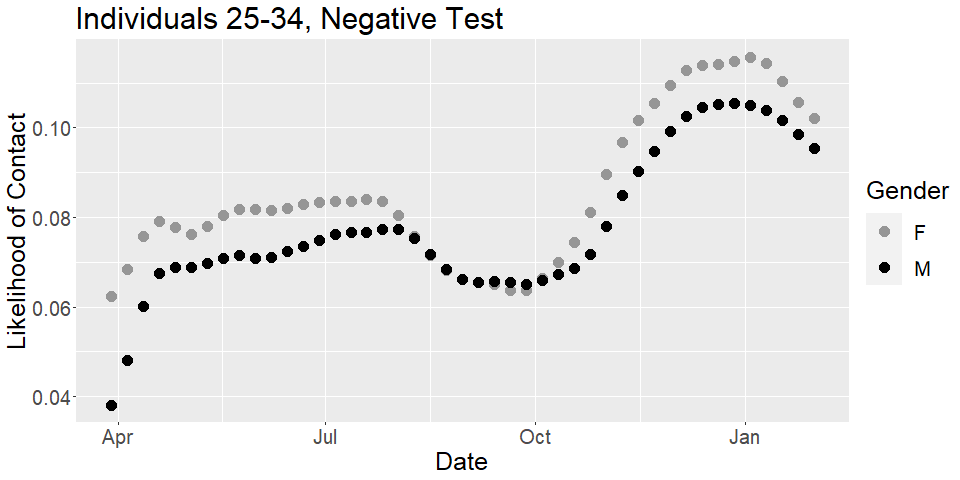
\includegraphics[width=.9\linewidth]{../figs/tvprop_contact_fig1.png}
 \caption{Contact Likelihood Given Negative Test}
 \label{fig:contactlik1}
\end{subfigure}%
\begin{subfigure}{.5\textwidth}
 \centering
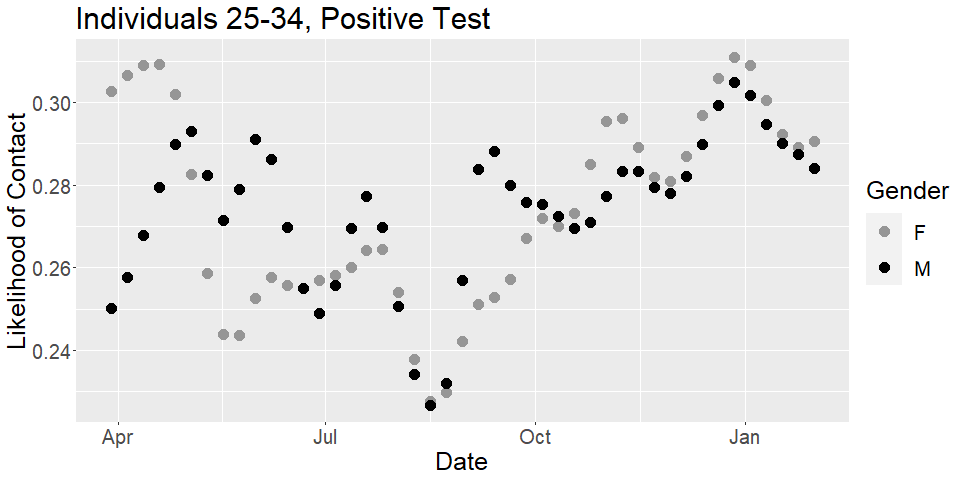
\includegraphics[width=.9\linewidth]{../figs/tvprop_contact_fig2.png}
 \caption{Contact Likelihood Given Positive Test}
 \label{fig:contactlik2}
\end{subfigure}
\caption{Likelihood of COVID-19 contact}
\label{fig:contactlik}
\end{figure}

We then use the pseudo-likelihood to compute the likelihood of fever given age, gender, COVID-19 contact status and test result.  Figure~\ref{fig:symptomlik1} and~\ref{fig:symptomlik2} plots the likelihood for 35-44 year olds given a negative test and positive test respectfully.  We see that the likelihood of fever depends heavily on whether they had a COVID-19 contact and their test results. Again, the likelihood is time-varying for most configurations.


\begin{figure}[!th]
\centering
\begin{subfigure}{.5\textwidth}
 \centering
 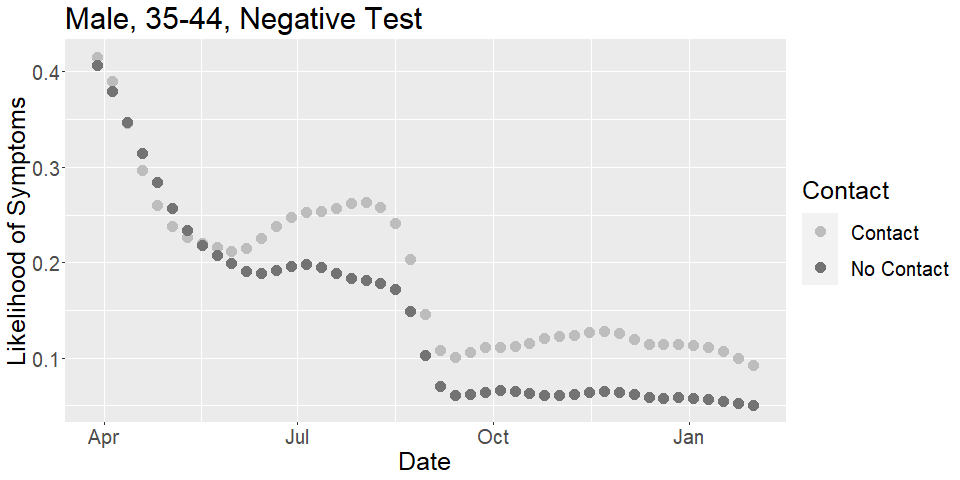
\includegraphics[width=.9\linewidth]{../figs/tvprop_symptom_fig1.png}
 \caption{Symptom Likelihood Given Negative Test}
 \label{fig:symptomlik1}
\end{subfigure}%
\begin{subfigure}{.5\textwidth}
 \centering
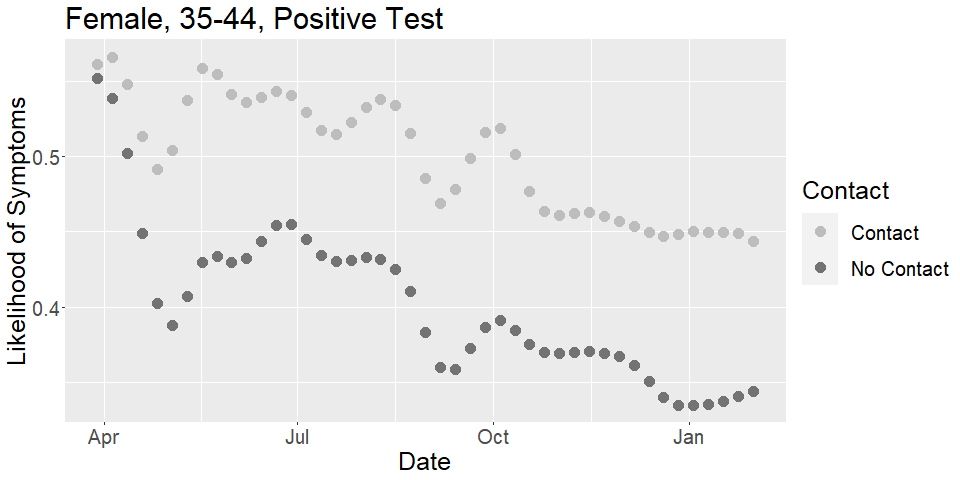
\includegraphics[width=.9\linewidth]{../figs/tvprop_symptom_fig2.png}
 \caption{Symptom Likelihood Given Positive Test}
 \label{fig:symptomlik2}
\end{subfigure}
\caption{Likelihood of reported COVID-19 symptoms}
\label{fig:symptomlik}
\end{figure}

Based on mean-imputation of COVID-19 contact and fever indicators, we can use the proposed pseudo-likelihood approach to compute the likelihood of getting tested for COVID-19 given age, ethnicity, race, gender, fever status, and COVID-19 contact indicator.  Figure~\ref{fig:testinglik1} and~\ref{fig:testinglik2} plots the likelihood of testing given fever and COVID-19 contact and no fever nor COVID-19 contact respectfully.  We see that the likelihood is time-varying and depends heavily on both fever and COVID-19 contact indicators.


\begin{figure}[!th]
\centering
\begin{subfigure}{.5\textwidth}
 \centering
 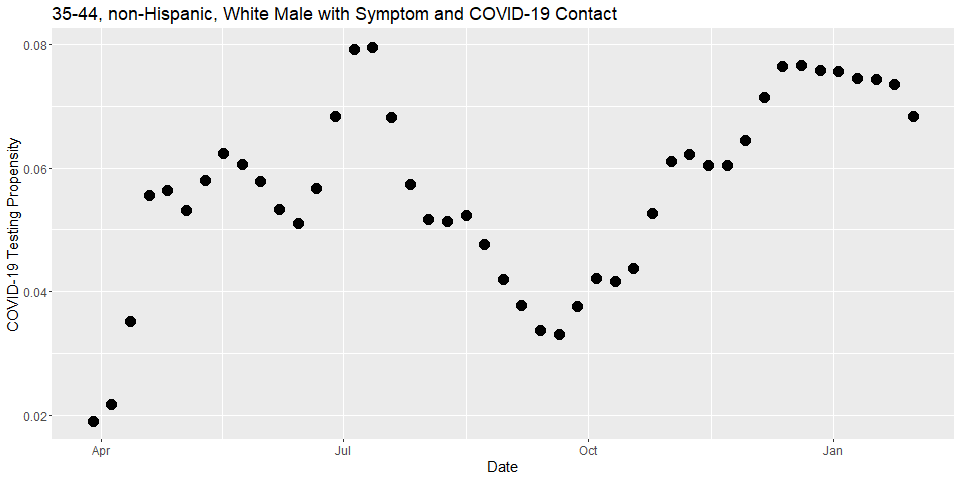
\includegraphics[width=.9\linewidth]{../figs/tvprop_fig1.png}
 \caption{Testing Likelihood Given Fever and \\COVID-19 Contact}
 \label{fig:testinglik1}
\end{subfigure}%
\begin{subfigure}{.5\textwidth}
 \centering
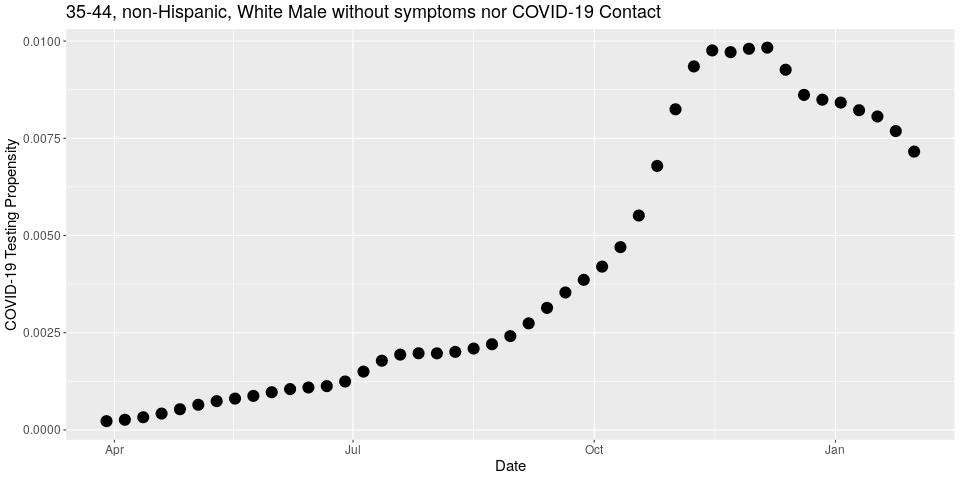
\includegraphics[width=.9\linewidth]{../figs/tvprop_fig2.png}
 \caption{Testing Likelihood Given no Fever nor \\  COVID-19 Contact}
 \label{fig:testinglik2}
\end{subfigure}
\caption{Testing Likelihood Given no Fever nor COVID-19 Contact}
\label{fig:testinglik}
\end{figure}

\subsection{Model 2 (Hospitalization)}

This model uses hospitalization records to try and improve our mean-imputation strategy.  First, we use the pseudo-likelihood to compute the likelihood of fever given age, gender, and test result.  The model only depends on hospitalization status for positive tests.  Figure~\ref{fig:symptomlik1_model2} and~\ref{fig:symptomlik2_model2} plots the likelihood for 35-44 years old given a negative test and positive test respectfully.  We see that the likelihood of fever is time-varying.  For a negative test, the likelihood of ever fever is very high in early April, which accounts for testing restrictions. We see that hospitalization significantly increases the risk of fever given a positive test.

\begin{figure}[!th]
\centering
\begin{subfigure}{.5\textwidth}
 \centering
 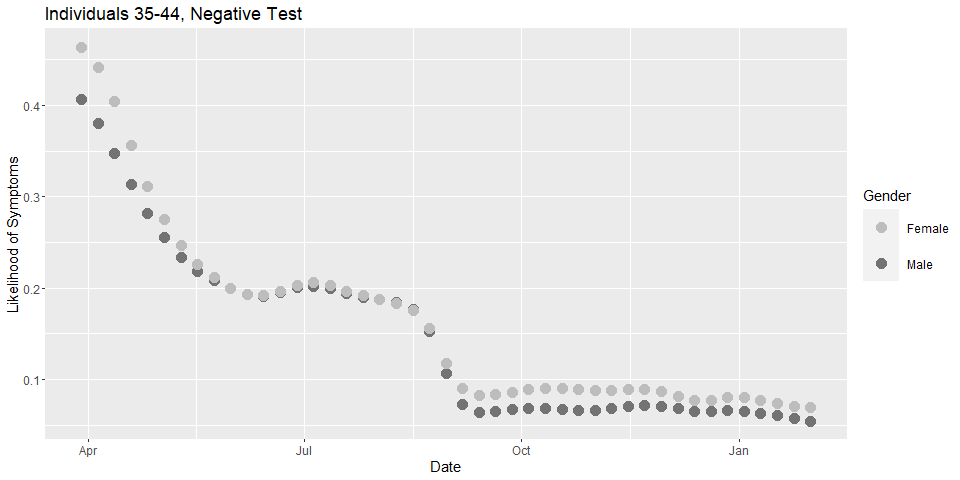
\includegraphics[width=.9\linewidth]{../figs/tvprop_symptom_alt_fig1.png}
 \caption{Symptom Likelihood Given Negative Test}
 \label{fig:symptomlik1_model2}
\end{subfigure}%
\begin{subfigure}{.5\textwidth}
 \centering
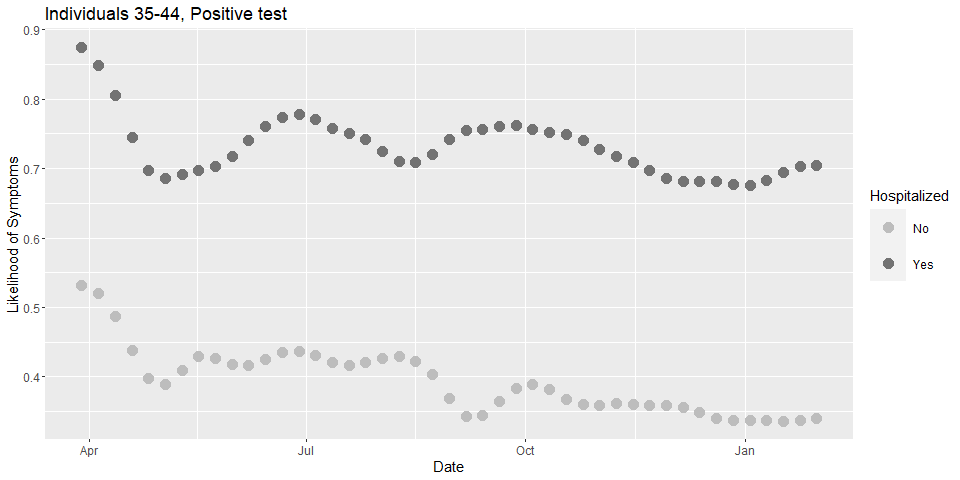
\includegraphics[width=.9\linewidth]{../figs/tvprop_symptom_alt_fig2.png}
 \caption{Symptom Likelihood Given Positive Test}
 \label{fig:symptomlik2_model2}
\end{subfigure}
\caption{Likelihood of COVID-19 contact}
\label{fig:symptomlik_model2}
\end{figure}

First, we computed the probability of fever given COVID-19 positive test and hospitalization as well as COVID-19 positive test and no hospitalization.  We then computed the likelihood of symptom given a COVID-19 positive test by weighting these two likelihoods by the fraction of COVID-19 positive hospitalizations to COVID-19 total positive cases per week.  Mean imputation of fever status for COVID-19 negative tests was performed based on the above model without use of hospitalization data.

Based on mean-imputation of COVID-19 fever using hospitalization records indicators, we can use the proposed pseudo-likelihood approach to compute the likelihood of getting tested for COVID-19 given age, ethnicity, race, gender, and fever status.  Figure~\ref{fig:testinglik1_mainpaper} and~\ref{fig:testinglik2_mainpaper} in Section~\ref{section:tvipw} of the manuscript plots the likelihood of testing given fever and no fever respectfully for all age ranges.  We see that the likelihood is time-varying and depends heavily on both fever status.

\subsubsection{Propensity plots}
\label{section:propplots}

Here we present the testing propensity for four strata: (1) non-Hispanic, white female, (2) non-Hispanic, African American male, (3) Hispanic, White male, and (4) Hispanic male who selects `Some other Race'.   Strata (1) presented in Figure~\ref{fig:nonh-white-female} demonstrates a small gender difference in testing propensities.  Strata (2) and (3) presented in Figures~\ref{fig:nonh-aa-male} and~\ref{fig:h-white-male} demonstrates a lower rate of testing among African Americans and Hispanic white men compared to non-Hispanic, white men respectively (approximately 2 times lower). Strata (4) presented in Figure~\ref{fig:h-other-male} demonstrates a much higher testing rate for Hispanic men who select ``Some Other Race''.

\begin{figure}[!th]
\centering
\begin{subfigure}{.5\textwidth}
 \centering
 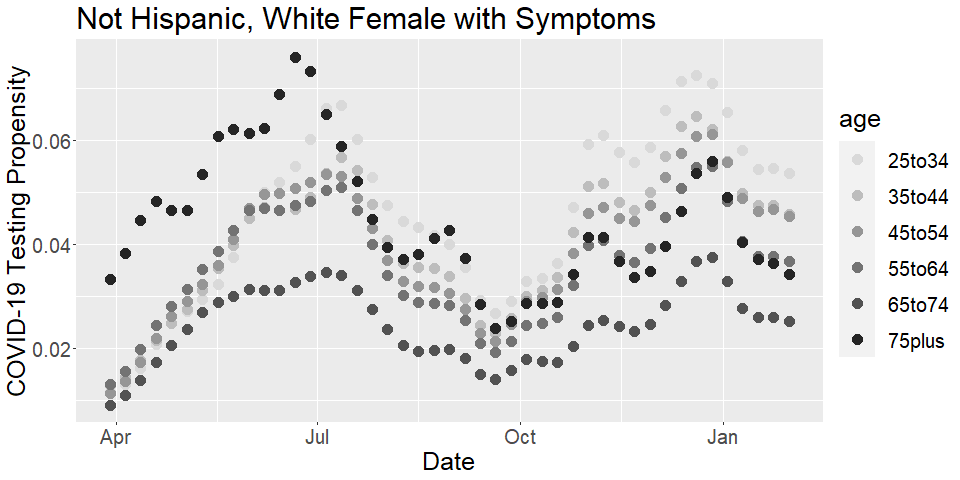
\includegraphics[width=.9\linewidth]{../figs/tvprop_alt_fig1_supp4.png}
 \caption{Symptom Likelihood Given Negative Test}
\end{subfigure}%
\begin{subfigure}{.5\textwidth}
 \centering
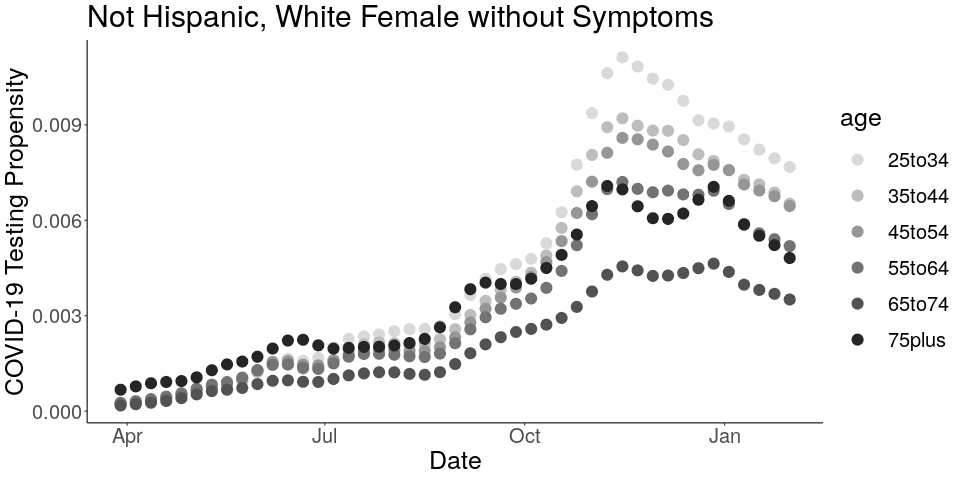
\includegraphics[width=.9\linewidth]{../figs/tvprop_alt_fig2_supp4.png}
 \caption{Symptom Likelihood Given Positive Test}
\end{subfigure}
\caption{Likelihood of COVID-19 contact for Non-Hispanic, White Females}
\label{fig:nonh-white-female}
\end{figure}

\begin{figure}[!th]
\centering
\begin{subfigure}{.5\textwidth}
 \centering
 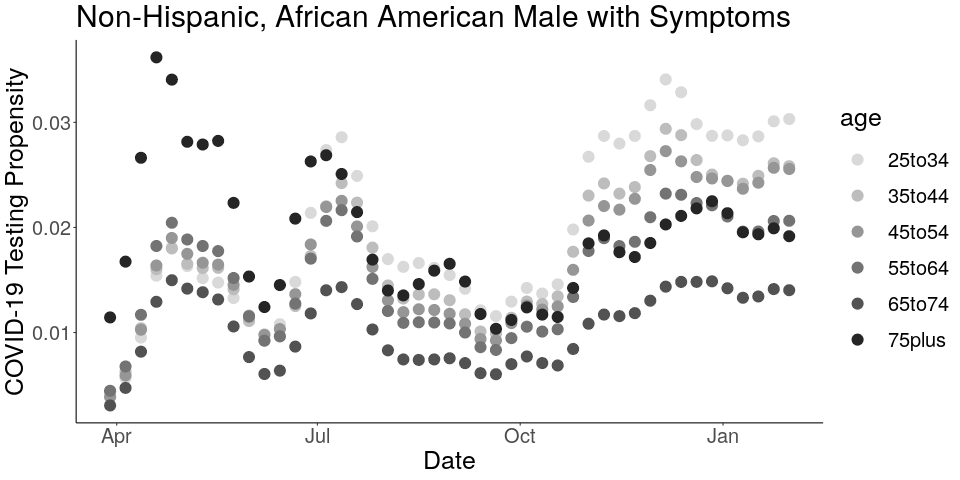
\includegraphics[width=.9\linewidth]{../figs/tvprop_alt_fig1_supp1.png}
 \caption{Symptom Likelihood Given Negative Test}
\end{subfigure}%
\begin{subfigure}{.5\textwidth}
 \centering
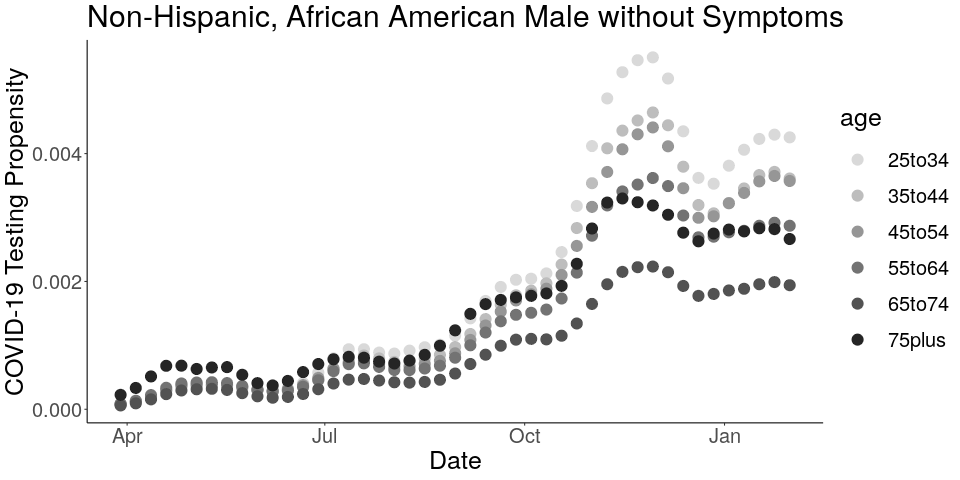
\includegraphics[width=.9\linewidth]{../figs/tvprop_alt_fig2_supp1.png}
 \caption{Symptom Likelihood Given Positive Test}
\end{subfigure}
\caption{Likelihood of COVID-19 contact for Non-Hispanic, African American Males}
\label{fig:nonh-aa-male}
\end{figure}

\begin{figure}[!th]
\centering
\begin{subfigure}{.5\textwidth}
 \centering
 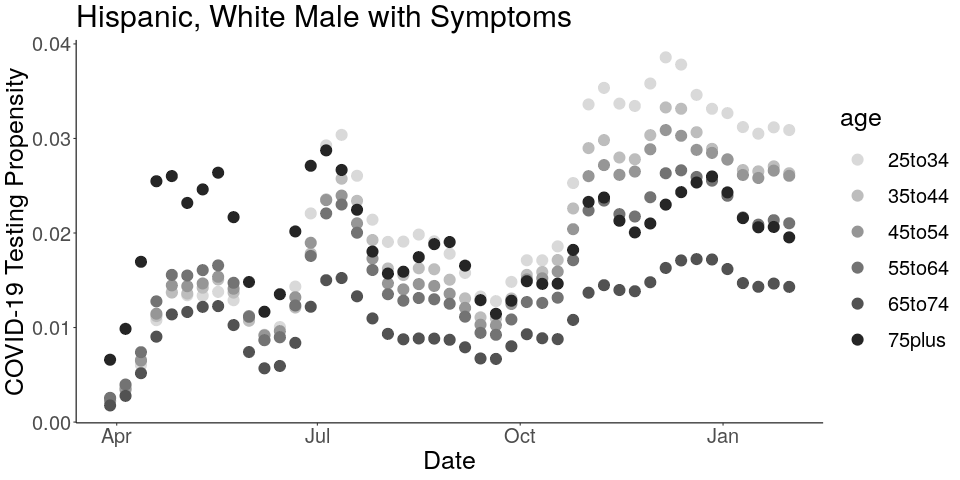
\includegraphics[width=.9\linewidth]{../figs/tvprop_alt_fig1_supp2.png}
 \caption{Symptom Likelihood Given Negative Test}
\end{subfigure}%
\begin{subfigure}{.5\textwidth}
 \centering
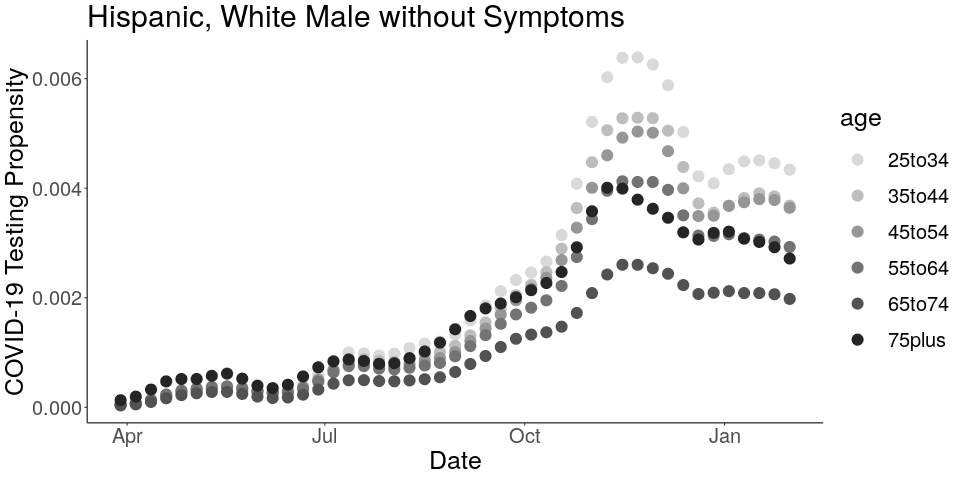
\includegraphics[width=.9\linewidth]{../figs/tvprop_alt_fig2_supp2.png}
 \caption{Symptom Likelihood Given Positive Test}
\end{subfigure}
\caption{Likelihood of COVID-19 contact for Hispanic, White Males}
\label{fig:h-white-male}
\end{figure}

\begin{figure}[!th]
\centering
\begin{subfigure}{.5\textwidth}
 \centering
 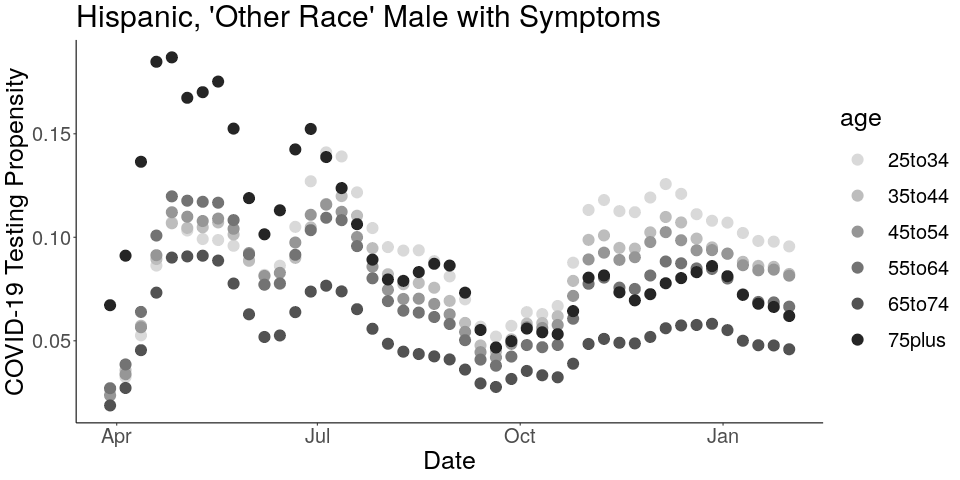
\includegraphics[width=.9\linewidth]{../figs/tvprop_alt_fig1_supp3.png}
 \caption{Symptom Likelihood Given Negative Test}
\end{subfigure}%
\begin{subfigure}{.5\textwidth}
 \centering
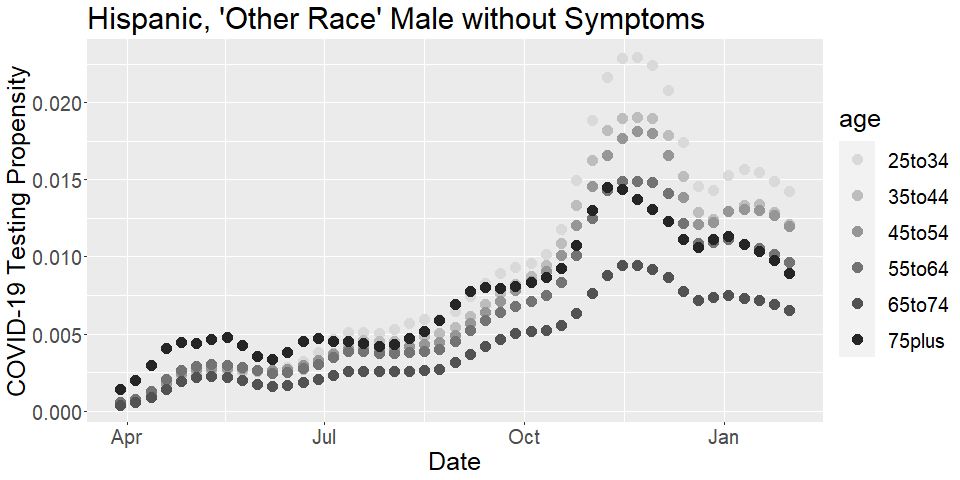
\includegraphics[width=.9\linewidth]{../figs/tvprop_alt_fig2_supp3.png}
 \caption{Symptom Likelihood Given Positive Test}
\end{subfigure}
\caption{Likelihood of COVID-19 contact for Hispanic, Males who select `Some Other Race'.}
\label{fig:h-other-male}
\end{figure}



\newpage
\subsubsection{Confidence Intervals}


Figure~\ref{fig:air_cis} in the supplementary materials presents the confidence intervals per time point for the IPW2 estimator.  The confidence interval length decreases substantially over time, reflecting the increased testing capacity.  Due to the number of surveys per week, under correct model specification there is minimal uncertainty in the parameter estimates.  As the number of tests per week increases to over one hundred thousand, there is minimal uncertainty in the active infection rate estimates. This points to the importance of the statistical decomposition~\eqref{eq:statdecomp2} and the discussion in Section~\ref{section:IPWerrordecomp}.

\begin{figure}[!th]
 \centering
 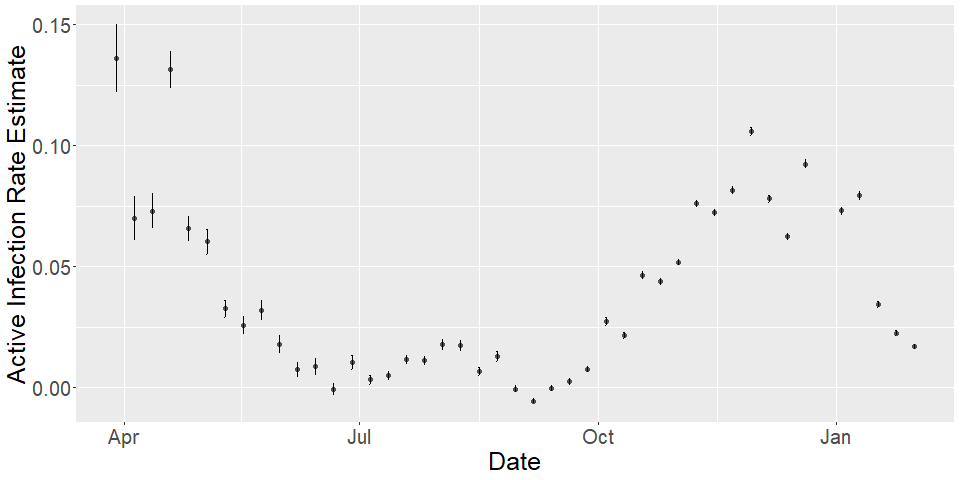
\includegraphics[width=.6\linewidth]{../figs/tv_air_cis.png}
 \caption{IPW2 estimate with confidence intervals}
 \label{fig:air_cis}
\end{figure}


% \begin{figure}[!th]
% \centering
% \begin{subfigure}{.5\textwidth}
%  \centering
%  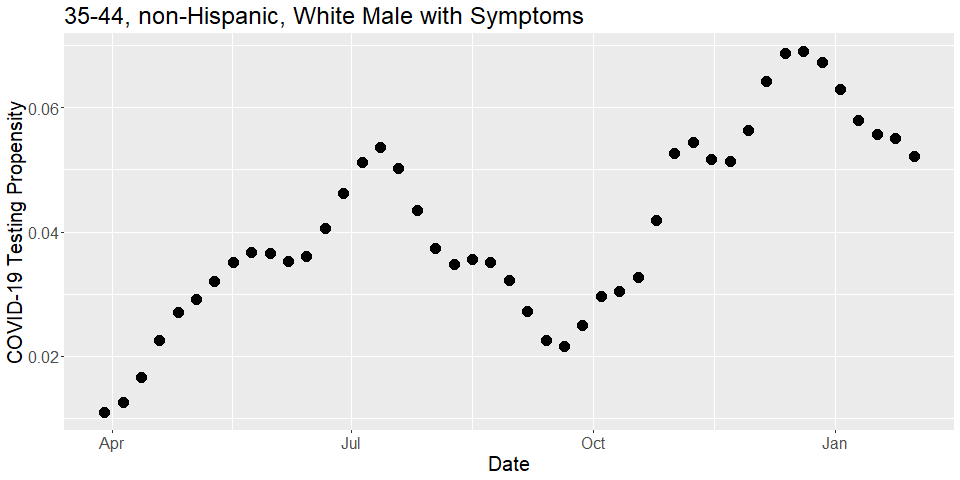
\includegraphics[width=.9\linewidth]{../figs/tvprop_alt_fig1.png}
%  \caption{Testing Likelihood Given Fever}
%  \label{fig:tvprop_alt_fig1.png}
% \end{subfigure}%
% \begin{subfigure}{.5\textwidth}
%  \centering
% 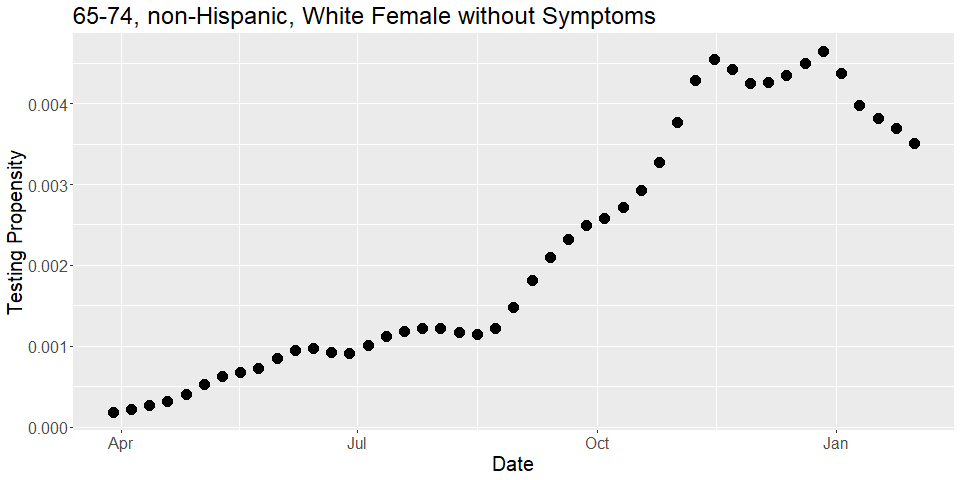
\includegraphics[width=.9\linewidth]{../figs/tvprop_alt_fig2.png}
%  \caption{Testing Propensity Given No Fever}
%  \label{fig:tvprop_alt_fig2.png}
% \end{subfigure}
% \caption{COVID-10 Testing Likelihood Given no Fever nor COVID-19 Contact}
% \label{fig:testinglik}
% \end{figure}

\section{Model-based: Prior specification}
\label{app:prior_modelbased}

For simplicity, we list the priors used in STAN below:
\begin{itemize}
  \item \code{beta $\sim$ Normal(1.5, 1) T[0,];}
  \item \code{gamma $\sim$ normal(0.3, 0.5) T[0,];}
  \item \code{sigma $\sim$ normal(0.4, 0.5) T[0,];}
  \item \code{phi\_inv $\sim$ exponential(5);}
  \item \code{i0 $\sim$ normal(0, 10);}
  \item \code{e0 $\sim$ normal(0, 10);}
  \item \code{eta $\sim$ normal(1, 1) T[0,];}
  \item \code{eta\_two $\sim$ normal(1, 1) T[0,];}
  \item \code{eta\_three $\sim$ normal(1, 1) T[0,];}
  \item \code{nu $\sim$ exponential(1./5);}
  \item \code{nu\_two $\sim$ exponential(1./5);}
  \item \code{nu\_three $\sim$ exponential(1./5);}
  \item \code{xi\_raw $\sim$ beta(1, 1);}
  \item \code{phi = 1/phi\_inv;}
  \item \code{xi = xi\_raw + 0.5;}
\end{itemize}
where \code{beta, eta, eta\_two, eta\_three} refer to the four values that form the time-varying parameter $\beta_t$ when combined with \code{xi, eta, eta\_two, eta\_three} in the SEIR model as described in Section~\ref{section:modelbased}. Following~\cite{Song2020}, we employ Runge-Kutta (RK4) approximations for discretization.  Due to the low number of deaths per strata, i.e., based on Race, Age, Sex and Ethnicity, we employ a kernel smoothing of the new infections per age strata into these sub-strata using relative number of observed deaths.  This ensured a suitably complex model that fits the observed death data well while generating strata-specific active infection rates that can be used in the doubly-robust estimation procedure.

\begin{figure}[!th]
 \centering
 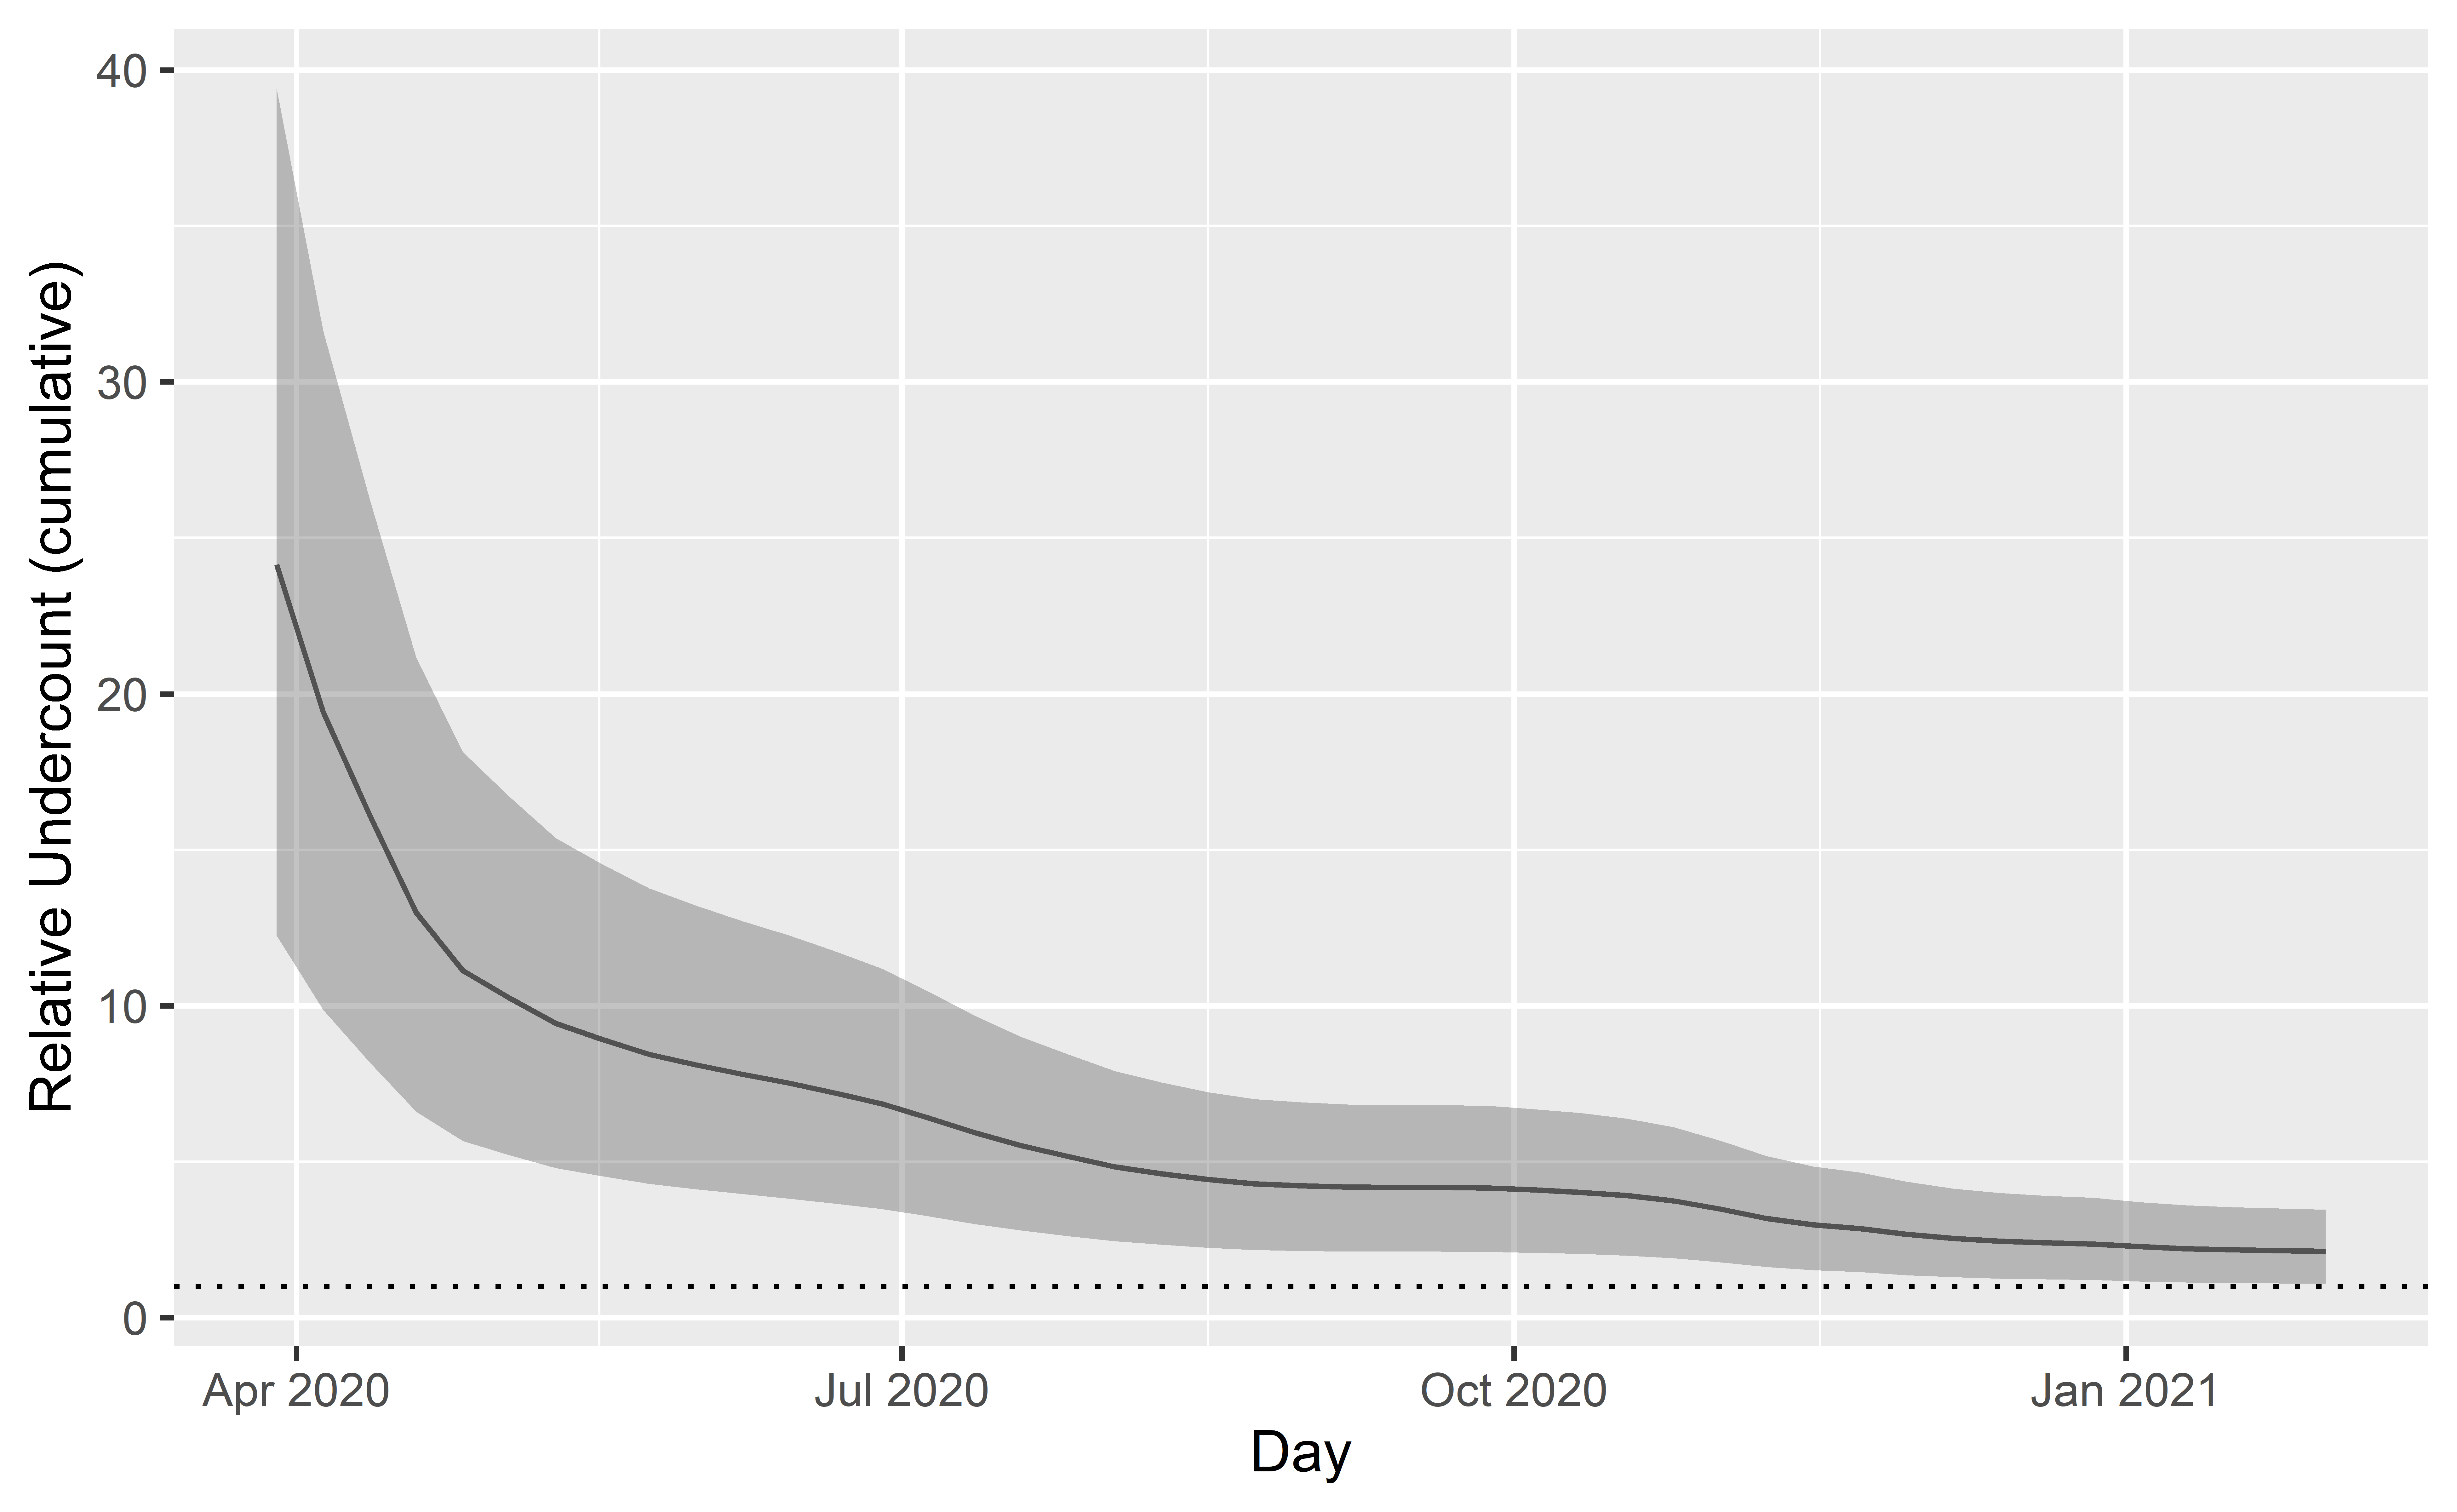
\includegraphics[width=.6\linewidth]{../figs/cumulative_undercounting.png}
 \caption{Cumulative undercount based on SEIR model}
 \label{fig:undercounting}
\end{figure}

Figure~\ref{fig:undercounting} is a plot of undercount based on the SEIR model.  We plot relative undercount on a cumulative basis since January due to the case counts reflecting active infections. Figure~\ref{fig:tv_air_sens} is a sensitivity analysis of the active infection rate under SEIR model with 10\% increase and decrease in the average IFR.  We see that the impact on the doubly robust estimates is minimal.



\begin{figure}[!th]
 \centering
 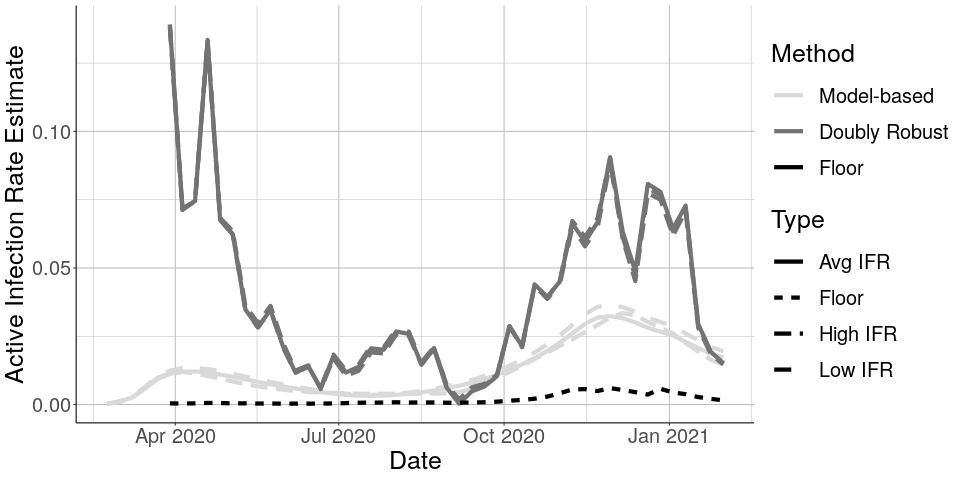
\includegraphics[width=.6\linewidth]{../figs/tv_air_sensitivity.png}
 \caption{Model-based and Doubly Robust active infection rate estimates under~\cite{Ironse2103272118} marginal IFR estimate of $0.84$\%, under a 10\% higher marginal IFR of $0.924$\%, and under a 10\% lower marginal IFR of $0.756$\%.}
 \label{fig:tv_air_sens}
\end{figure}

\section{Alternative estimator of the instantaneous reproductive number}
\label{app:cori_rt}

Here we present estimates of the instantaneous reproductive number using the approach of~\cite{Cori20113} under the SEIR model from Section~\ref{section:r0-estimation}.  Let~$I_t$ denote the total infectiousness of infected individuals at time~$t$.  Then~$E[I_t] = R_t \sum_{s=1}^{t} I_{t-s} w_s$ where $w_{u}$ is the infectivity function.  Here, we follow~\cite{Cori20113} and choose a discretized shifted Gamma distribution with mean $7$ days and standard deviation $2$ days.  Then a moment-based estimator can be obtained by $\hat R_t = I_t / \sum_{s=1}^t I_{t-s} w_s$, which takes the form of the ratio estimators in Section~\ref{section:rates}.  Therefore, the bias can be readily obtained from the associated Taylor series decomposition, with the terms related to time~$t-1$ replaced by a weighted version.  Figure~\ref{fig:cori-bias} presents the bias.


\begin{figure}
 \centering
  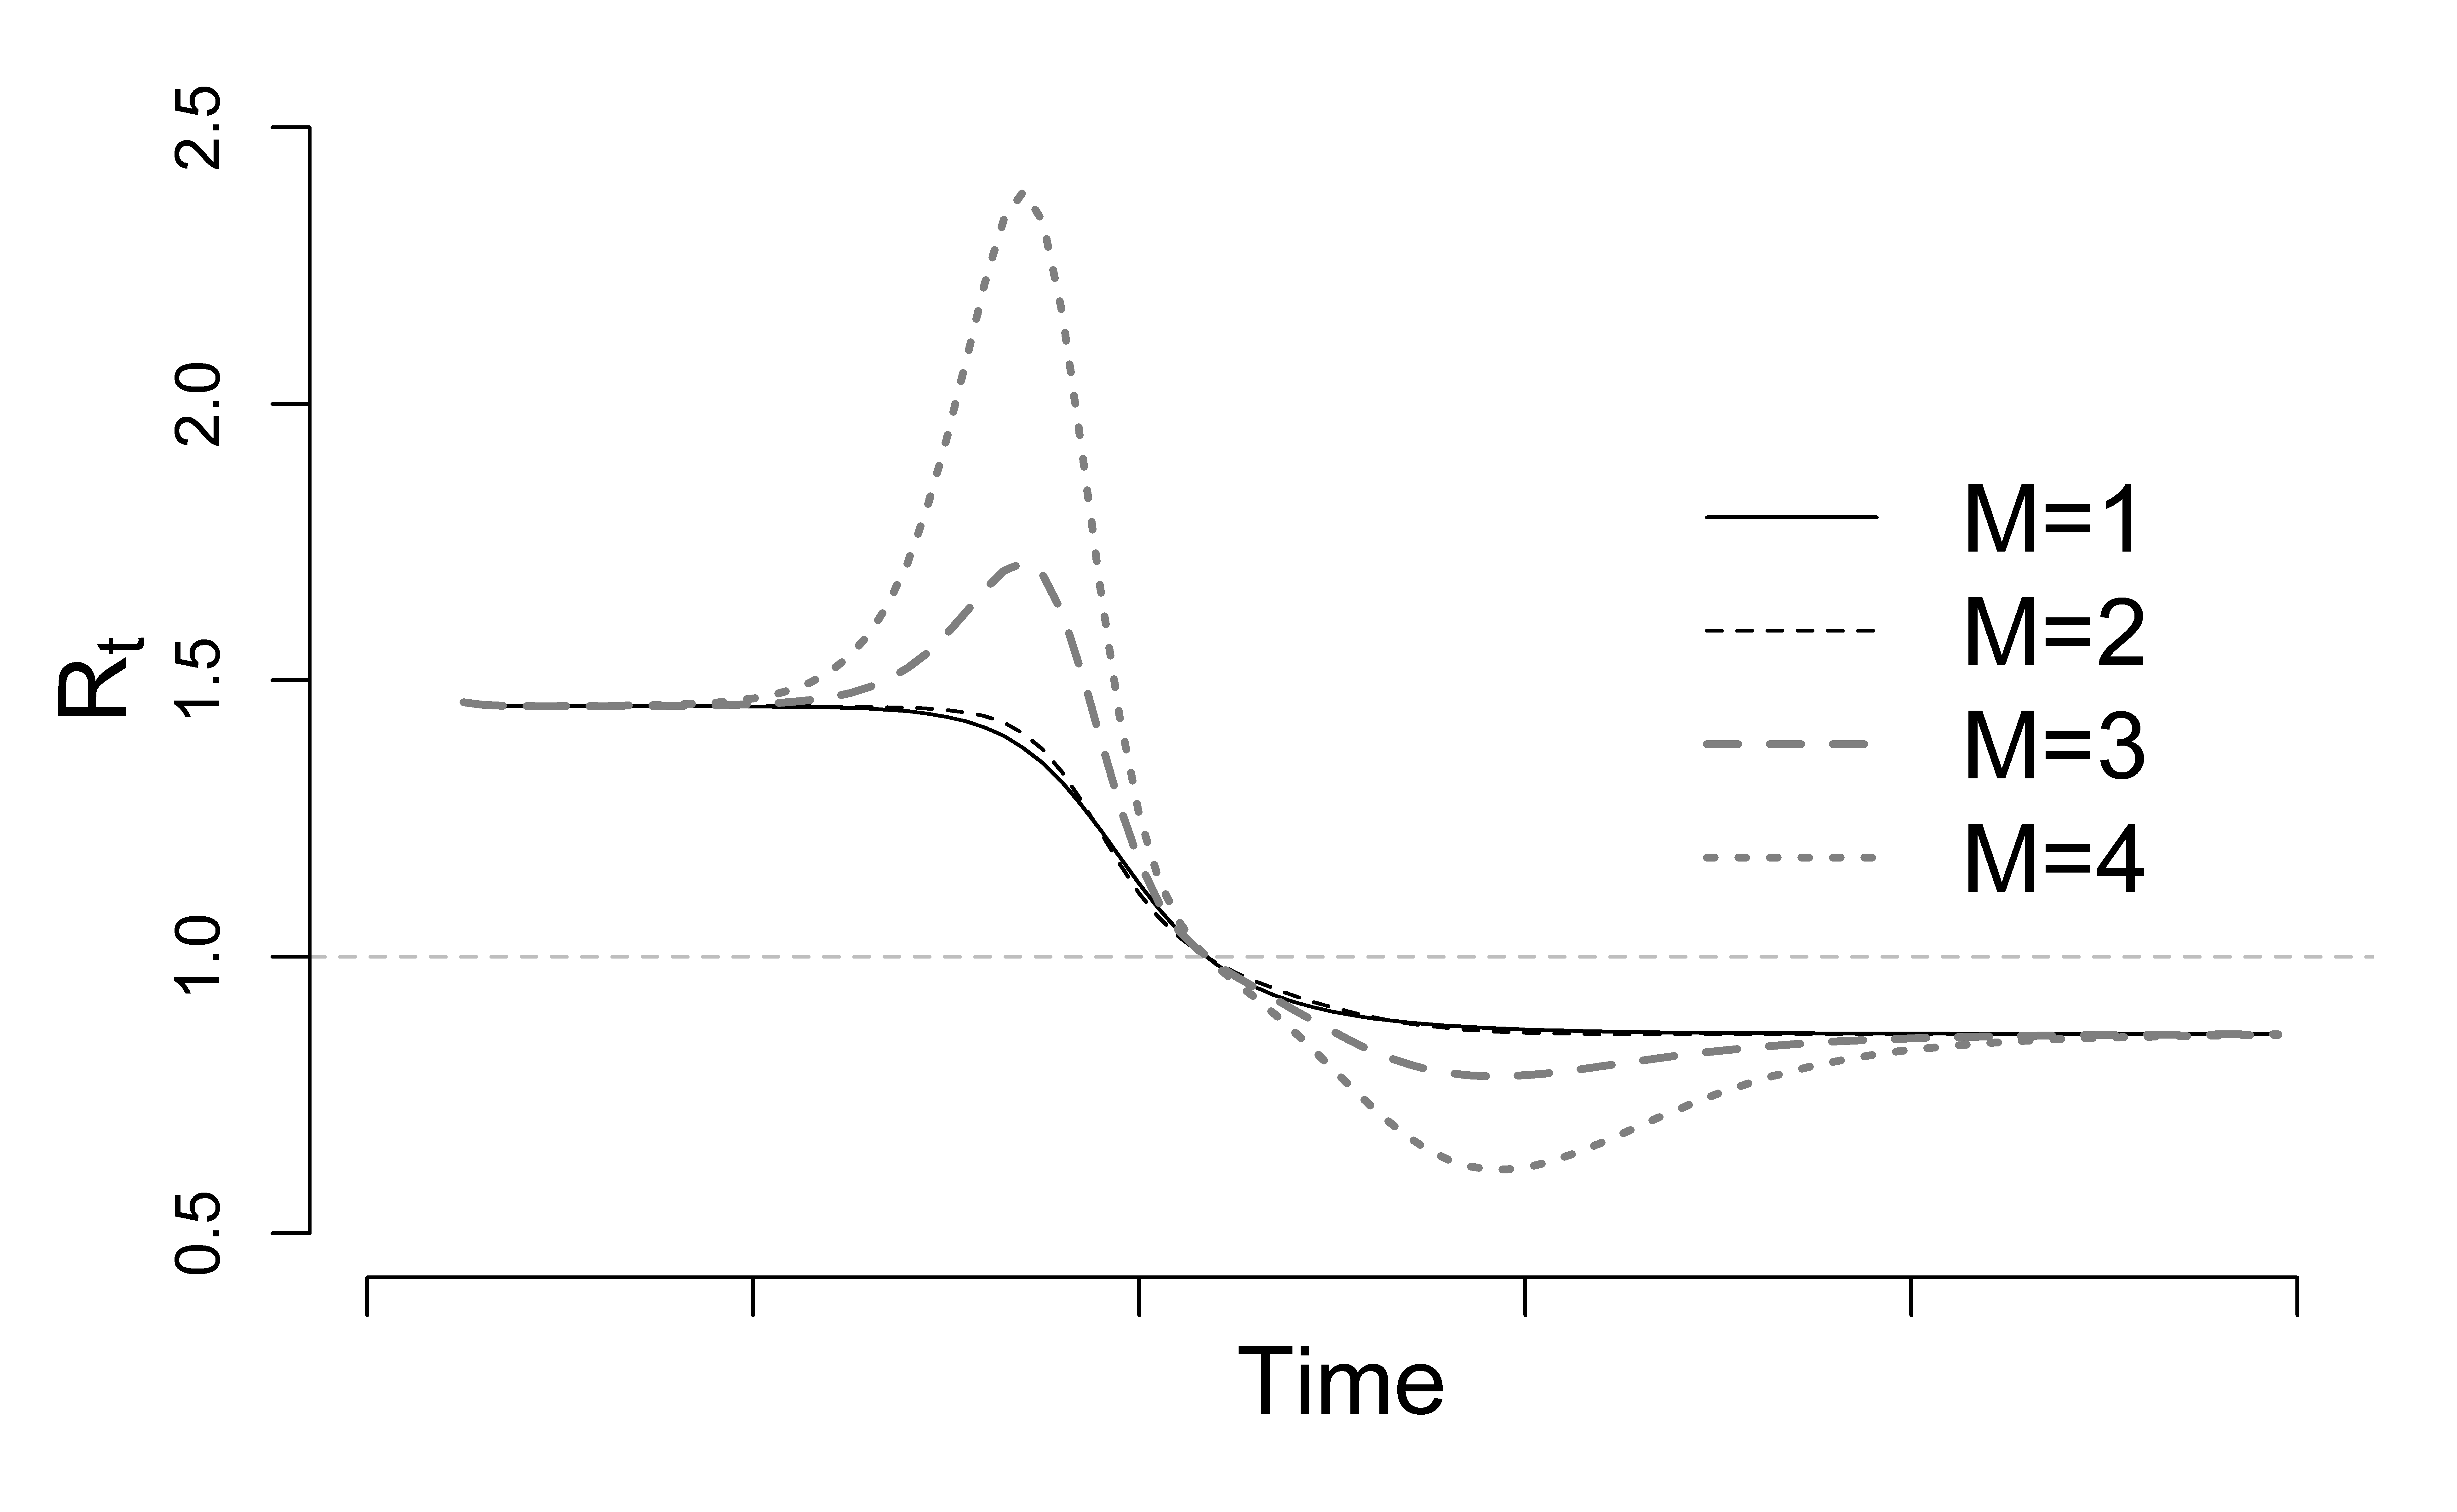
\includegraphics[width=.9\linewidth]{../figs/seir_cori_rt.png}
  \caption{Effective reproductive rate estimator}
 \caption{Potential bias in instantaneous reproductive rate estimator based on~\cite{Cori20113} under an SEIR model with $\beta = 1.2$, $\gamma = 0.15$, and $\sigma = 0.3$.  Here, $f = 0.02$, $FP = 0.024$, $FN = 0.13$, and a range of relative sampling fractions $M = f_1/f_0$ are considered.}
 \label{fig:cori-bias}
 \end{figure}


Figure~\ref{fig:cori-bias} presents the potential bias in instantaneous reproductive rate estimator.  The general conclusions follow similarly as in  Figure~\ref{fig:ratio-bias}. The rate is overestimated prior to the peak and underestimated afterwards.  Estimates at the peak time appear to have minimal bias.

\section{Sensitivity Analysis}

The proposed approach relies on the assumption $I_{j,t}^{(NR)} \indep Y_{j,t} \, | \, X_{j,t}$, i.e., the sampling indicator in the non-probabilistic survey is conditionally independent of the outcome given the covariates.  However, estimates of population quantities based on inverse-weighting and/or model-based estimates will be biased in the presence of `unobserved confounding'.  The purpose of this section is to introduce a sensitivity analysis to address this concern.  To this end, we consider the logit-linear model by~\cite{Imbens2003}, adjusted to the time-varying, self-selection setting from the single time-point, causal inference setting.  That is, consider the model
\begin{align*}
\logit \pi \left( I_{t} = 1  | x_{t}, u_{t} \right) &= h_t(x_t) + \alpha_t u_t \\
E[ Y_t | i_t, x_t, u_t] &= l_t(i_t, x_t) + \delta_t u_t
\end{align*}
for some functions~$h_t$ and $l_t$ that are allowed to depend on time. Re-arranging the terms we see that
$$
E[ Y_t | i_t x_t, u_t ] = l_t(i_t,x)  + \frac{\delta_t}{\alpha_t} \left( \logit \pi \left( I_{t} = 1  | x_{t}, u_{t} \right) - h_t (x_t) \right)
$$
The key idea in~\cite{Imbens2003} is that positing a distribution on $\pi(I_t = 1 | x_y, u_t)$ directly allows one to circumvent the need to specify a distribution for~$U_t$, a highly non-trivial task.

The logit-linear model above unfortunately does not lead to a tractable sensitivity analysis.  Instead, we consider a sensitivity model based on work by~\cite{Veitch2020}, again adjusted to deal with the current setting of self-selection, given by:
\begin{equation}
\begin{aligned}
\label{eq:sensmodel}
\pi_t(X_t, U_t) &\sim \text{Beta} \left( \pi_t (X_t) (1/\alpha_t - 1), (1-\pi_t(X_t)) (1/\alpha_t - 1) \right) \\
I_t | X_t, U_t &\sim \text{Bern} (\pi (X_t,U_t)) \\
\rho_t(X_t, U_t) &= Q_t(X_t,1) + \delta_t \left( \logit \pi_t(X_t,U_t) - \EE \left[ \logit \pi_t(X_t,U_t) | X_t, I_t = 1 \right] \right) \\
Y_t | I_t, X_t, U_t &\sim \text{Bern}(\rho_t(X_t, U_t))
\end{aligned}
\end{equation}
The time-varying sensitivity parameter~$\alpha_t \in (0,1)$  controls the influence of the unobserved confounder~$U_t$ on selection propensity. In particular, $\alpha_t$ measures the change in belief of how likely an individual self-selects into the non-probabilistic sample at time~$t$:
$$
\alpha_t = E[ \pi_t (X_t,U_t) | I = 1] - E[ \pi_t (X_t,U_t) | I = 0].
$$
The sensitivity model satisfies the requirement that the self-selection propensity and conditional expectation outcome model can match the observed data:
\begin{align*}
P(I_t = 1 | X_t ) &= E[ E[ I_t | X_t, U_t ] | X_t ] = E[ \pi_t(X_t, U_t) | X_t ] = \pi_t (X_t) \\
E[Y_t = 1 | X_t, I_t = 1 ] &= E[ E[ Y_t | X_t, U_t, I_t =1 ] | X_t, I_t = 1 ] =: Q_t(1,X_t).
\end{align*}
Moreover, the model satisfies that $Y_t$ does not depend on $I_t$ given $(X_t, U_t)$. This is a key adaptation to the non-probabilistic survey setting with potential time-varying confounding and a binary outcome.

\noindent {\bf IPW estimator:} By assumption, observing $X_t$ and $U_t$ together leads to consistent estimation via the estimator:
\begin{align*}
\EE\left[\pi^{-1}_t (X_{J,t}, U_{J,t}) I_{J,t} Y_{J,t} \right]
= &\EE[ E[ Y_{J,t} | X_{J,t}, U_{J,t}] ] \\
= &\EE \left[ Q(1,X_{J,t}) + \delta \left( \logit \pi_t (X_{J,t}, U_{J,t}) - \EE \left[ \logit \pi_t (X_{J,t}, U_{J,t}) | X_{J,t}, I_{J,t} = 1 \right] \right) \right]
\end{align*}
\noindent {\bf IPW-based estimator:} Investigating the IPW estimator using only~$X_t$, we have:
\begin{align*}
\EE\left[\pi^{-1}_t (X_{J,t}) I_{J,t} Y_{J,t} \right]
=&\EE\left[\frac{\pi_t (X_{J,t}, U_{J,t})}{\pi_t (X_{J,t})} \pi^{-1} (X_{J,t}, U_{J,t}) I_{J,t} Y_{J,t} \right] \\
= &\EE\left[ \frac{\pi_t (X_{J,t}, U_{J,t})}{\pi_t (X_{J,t})} \EE[ Y_{J,t} | X_{J,t}, U_{J,t}] \right].
\end{align*}
Using the fact that $\EE \left[ \pi_t (X_{J,t}, U_{J,t}) | X_{J,t} \right] = \pi_{t} (X_{J,t})$, the \emph{bias} is
$$
\delta \EE \left[ \logit \pi_t (X_{t,J}, U_{t,J}) - \frac{\pi_t (X_{J,t}, U_{J,t})}{\pi_t (X_{J,t})} \logit \pi_t (X_{t,J}, U_{t,J}) \right].
$$
Using the fact that~$Z \sim Beta(\alpha, \beta)$ then $E[ ln(Z) ] = \psi(\alpha) - \psi(\alpha + \beta)$, $E[ ln(1-Z) ] = \psi(\beta) - \psi(\alpha + \beta)$ then~$E[ \logit (Z) ] = \psi(\alpha) - \psi(\beta)$ where~$\psi$ is the digamma function.  Moreover,~$\EE[ Z ln Z ] = \frac{\alpha}{\alpha + \beta} \left[ \psi(\alpha + 1) - \psi(\alpha + \beta +1) \right]$ and
\begin{align*}
\EE \left[ (1-Z) ln(1-Z) \right] &= \frac{\beta}{\alpha + \beta} \left[ \psi(\beta + 1) - \psi(\alpha + \beta +1) \right] \\
\EE \left[ ln(1-Z) \right] &= \left[ \psi(\beta) - \psi(\alpha + \beta) \right] \\
\Rightarrow - \EE \left[ Z ln(1-Z) \right] &= \frac{\beta}{\alpha + \beta} \left[ \psi(\beta + 1) - \psi(\alpha + \beta +1) \right] - \left[ \psi(\beta) - \psi(\alpha + \beta) \right].
\end{align*}
and thus
\begin{align*}
\EE \left[ Z \logit(Z) \right] =& \frac{\alpha}{\alpha + \beta} \left[ \psi(\alpha + 1) - \psi(\alpha + \beta +1) \right] + \frac{\beta}{\alpha + \beta} \left[ \psi(\beta + 1) - \psi(\alpha + \beta +1) \right] \\
&- \left[ \psi(\beta) - \psi(\alpha + \beta) \right] \\
=& \psi(\alpha + \beta) - \psi(\alpha + \beta +1) + \frac{\alpha}{\alpha + \beta} \left[ \psi(\alpha + 1) - \psi(\beta+1) \right] + \frac{1}{\beta} \\
=& \frac{\alpha}{\alpha + \beta} \left[ \psi(\alpha + 1) - \psi(\beta+1) \right] + \left[ \frac{1}{\beta} - \frac{1}{\alpha + \beta} \right].
\end{align*}
Plugging in $\alpha = \pi_t (X_t) (1/\alpha_t -1)$ and $\beta = (1-\pi_t (X_t))(1/\alpha_t - 1)$ yields:
$$
\pi_t (X_{t,J}) \left[ \psi \left(\pi_t (X_{t,J}) \left(\frac{1-\alpha_t}{\alpha_t}\right) + 1\right) - \psi \left((1-\pi_t (X_{t,J})) \left(\frac{1-\alpha_t}{\alpha_t}\right)+1\right) \right] + \frac{\alpha_t}{1-\alpha_t}\frac{\pi_t(X_{t,J})}{1-\pi_t(X_{t,J})}.
$$
Since $\pi_t(X_t)$ cancels with the denominator term, the first term will match the form of the $E[ \logit (Z)]$ and therefore using the fact that $\psi(x+1) = \psi(x) + 1/x$, we can write the bias simply as
$$
-\delta_t \frac{\alpha_t}{1-\alpha_t} \EE \left[ \frac{1}{\pi_t(X_{t,J})} \right]
$$
Note that this is an expectation over the population-level distribution of the covariate~$X$.  Thus, computation requires use of the probabilistic sample in order to estimate the potential bias.

% \noindent {\bf Model-based estimator:} Investigating the model-based estimator, we have:
% $$
% \EE\left[ E[ Y_{J,t} | X_{J,t}, I_{J,t} = 1] \right] = \EE\left[ Q(X_{J,t}, 1) \right]
% $$
% and so the bias is given by
% $$
% \delta \EE \left[ \left( \logit \pi_t (X_{J,t}, U_{J,t}) - \EE \left[ \logit \pi_t (X_{J,t}, U_{J,t}) | X_{J,t}, I_{J,t} = 1 \right] \right) \right]
% $$
% Using the above argument and the Beta-Bernoulli conjugacy we can re-write the bias as
% \begin{align*}
% \delta \EE \bigg[ &\psi \left( \frac{1-\alpha_t}{\alpha_t} \pi_t(X_{J,t}) \right) - \psi \left( \frac{1-\alpha_t}{\alpha_t} \left( 1 - \pi_t(X_{J,t}) \right) \right) \\
% &- \EE \bigg[ \psi \left( \frac{1-\alpha_t}{\alpha_t} \pi_t(X_{J,t}) + 1 \right) - \psi \left(\frac{1-\alpha_t}{\alpha_t} \left( 1 - \pi_t(X_{J,t}) \right) \right) \big | X_{J,t}, I_{J,t} = 1 \bigg] \bigg]
% \end{align*}
% Note that the 2nd expectation is over the distribution of $X$ conditional on response~$I=1$ while the first is not conditional.  Therefore, the first expectation requires use of the random sample for computation while the second expectation requires use of the non-probabilistic sample.  If the distribution of $X$ were independent of $I$ then the bias would simplify to
% $$
% -\delta_t \frac{1-\alpha_t}{\alpha_t} \EE \left[ \frac{1}{\pi_t (X_t)} \right].
% $$
% which is exactly equal to the IPW estimator bias.  In settings where $X$ strongly depends on $I$ this is not the case.

\subsection{Reparametrization}

Following~\cite{Veitch2020}, we re-express the outcome-confounder strength in terms of the partial coefficient of determination
$$
R_Y^2 (\alpha, \delta) = \frac{\EE [( Y - Q(1,X) )^2 | I=1 ] - \EE[ (Y - \EE[ Y | X, U ])^2]}{E[(Y - Q(1,X))^2 | I = 1]}
$$
in terms of $\delta^2$.  To do so, writ
em\begin{align*}
\EE [ (Y - \EE[ Y | X, U] )^2 | I = 1 ] =& \EE [ (Y - Q(1,X))^2 | I = 1 ] \\
&- 2 \delta \EE \left[ (Y - Q(1,X)) (\logit \pi(X,U) - \EE[ \logit \pi (X,U) | X, I=1 ]) | I = 1 \right] \\
&+ \delta^2 \EE \left[ (\logit \pi(X,U) - \EE[ \logit \pi (X,U) | X, I=1 ])^2 | I = 1 \right] \\
&= \EE [ (Y - Q(1,X))^2 | I = 1 ] - \delta^2 \EE \left[ \text{var} \left( \logit \pi(X,U) \right) | X, I = 1 \right]
\end{align*}
By Beta-Bernoulli conjugacy, the second term is the variance of the logit-transformed Beta distribution which has an analytic expression:
$$
\text{var} \left( \logit \pi(X,U) | X, I = 1 \right) = \psi_1 ( \pi(X) (\alpha - 1) + 1 ) + \psi_1 ( (1- \pi(X)) (1/\alpha - 1))
$$
where $\psi_1$ is the trigamma function. This implies the outcome influence is
$$
R_Y^2 (\alpha, \delta) = \delta^2 \frac{\EE [\psi_1 ( \pi(X) (\alpha - 1) + 1 ) + \psi_1 ( (1- \pi(X)) (1/\alpha - 1))] }{E [(Y- Q(1,X))^2 | I = 1]}
$$
Note this expectation is over those who

Following from~\cite[Theorem 5]{Veitch2020}, the parameter~$\alpha$ can be reexpressed in a more convenient form:
$$
\alpha = 1 - \frac{\EE \left[ \pi (X_{t,J},U_{t,J}) \left( 1 - \pi (X_{t,J},U_{t,J}) \right)  \right]}{\EE\left[ \pi (X_{t,J}) \left( 1 - \pi (X_{t,J}) \right) \right] }
$$

\subsection{Estimating sensitivity parameters}

Based on equations XX and XX, we can estimate the time-varying sensitivity parameters.

With these estimates







\bibliographystyle{plainnat}
\bibliography{covid-refs}



\end{document}